\documentclass[]{book}
\usepackage{lmodern}
\usepackage{amssymb,amsmath}
\usepackage{ifxetex,ifluatex}
\usepackage{fixltx2e} % provides \textsubscript
\ifnum 0\ifxetex 1\fi\ifluatex 1\fi=0 % if pdftex
  \usepackage[T1]{fontenc}
  \usepackage[utf8]{inputenc}
\else % if luatex or xelatex
  \ifxetex
    \usepackage{mathspec}
  \else
    \usepackage{fontspec}
  \fi
  \defaultfontfeatures{Ligatures=TeX,Scale=MatchLowercase}
\fi
% use upquote if available, for straight quotes in verbatim environments
\IfFileExists{upquote.sty}{\usepackage{upquote}}{}
% use microtype if available
\IfFileExists{microtype.sty}{%
\usepackage{microtype}
\UseMicrotypeSet[protrusion]{basicmath} % disable protrusion for tt fonts
}{}
\usepackage[margin=1in]{geometry}
\usepackage{hyperref}
\hypersetup{unicode=true,
            pdftitle={Calcul différentiel et intégral dans l'espace},
            pdfauthor={Marc-André Désautels},
            pdfborder={0 0 0},
            breaklinks=true}
\urlstyle{same}  % don't use monospace font for urls
\usepackage{natbib}
\bibliographystyle{apalike}
\usepackage{longtable,booktabs}
\usepackage{graphicx,grffile}
\makeatletter
\def\maxwidth{\ifdim\Gin@nat@width>\linewidth\linewidth\else\Gin@nat@width\fi}
\def\maxheight{\ifdim\Gin@nat@height>\textheight\textheight\else\Gin@nat@height\fi}
\makeatother
% Scale images if necessary, so that they will not overflow the page
% margins by default, and it is still possible to overwrite the defaults
% using explicit options in \includegraphics[width, height, ...]{}
\setkeys{Gin}{width=\maxwidth,height=\maxheight,keepaspectratio}
\IfFileExists{parskip.sty}{%
\usepackage{parskip}
}{% else
\setlength{\parindent}{0pt}
\setlength{\parskip}{6pt plus 2pt minus 1pt}
}
\setlength{\emergencystretch}{3em}  % prevent overfull lines
\providecommand{\tightlist}{%
  \setlength{\itemsep}{0pt}\setlength{\parskip}{0pt}}
\setcounter{secnumdepth}{5}
% Redefines (sub)paragraphs to behave more like sections
\ifx\paragraph\undefined\else
\let\oldparagraph\paragraph
\renewcommand{\paragraph}[1]{\oldparagraph{#1}\mbox{}}
\fi
\ifx\subparagraph\undefined\else
\let\oldsubparagraph\subparagraph
\renewcommand{\subparagraph}[1]{\oldsubparagraph{#1}\mbox{}}
\fi

%%% Use protect on footnotes to avoid problems with footnotes in titles
\let\rmarkdownfootnote\footnote%
\def\footnote{\protect\rmarkdownfootnote}

%%% Change title format to be more compact
\usepackage{titling}

% Create subtitle command for use in maketitle
\newcommand{\subtitle}[1]{
  \posttitle{
    \begin{center}\large#1\end{center}
    }
}

\setlength{\droptitle}{-2em}

  \title{Calcul différentiel et intégral dans l'espace}
    \pretitle{\vspace{\droptitle}\centering\huge}
  \posttitle{\par}
    \author{Marc-André Désautels}
    \preauthor{\centering\large\emph}
  \postauthor{\par}
      \predate{\centering\large\emph}
  \postdate{\par}
    \date{2018-09-26}

\usepackage{booktabs}
\usepackage{tcolorbox}
\usepackage{amsthm}
\usepackage{multido}
\usepackage[french]{babel}

\hypersetup{colorlinks=true, urlcolor=blue}

\renewcommand{\chaptername}{Chapitre}
\renewcommand{\contentsname}{Table des Matières}
\renewcommand{\partname}{Partie}
\renewcommand\bibname{Bibliographie}

\newenvironment{exemple}{\begin{tcolorbox}\begin{example}}{\end{example}\end{tcolorbox}}

\usepackage{amsthm}
\newtheorem{theorem}{Théorème}[chapter]
\newtheorem{lemma}{Lemme}[chapter]
\newtheorem{corollary}{Corollaire}[chapter]
\newtheorem{proposition}{Proposition}[chapter]
\newtheorem{conjecture}{Conjecture}[chapter]
\theoremstyle{definition}
\newtheorem{definition}{Définition}[chapter]
\theoremstyle{definition}
\newtheorem{example}{Exemple}[chapter]
\theoremstyle{definition}
\newtheorem{exercise}{Exercice}[chapter]
\theoremstyle{remark}
\newtheorem*{remark}{Remarque}
\newtheorem*{solution}{Solution}
\let\BeginKnitrBlock\begin \let\EndKnitrBlock\end
\begin{document}
\maketitle

{
\setcounter{tocdepth}{2}
\tableofcontents
}
\hypertarget{introduction}{%
\chapter*{Introduction}\label{introduction}}
\addcontentsline{toc}{chapter}{Introduction}

\hypertarget{a-propos-de-ce-document}{%
\section*{À propos de ce document}\label{a-propos-de-ce-document}}
\addcontentsline{toc}{section}{À propos de ce document}

\hypertarget{remerciements}{%
\subsection*{Remerciements}\label{remerciements}}
\addcontentsline{toc}{subsection}{Remerciements}

Ce document est généré par l'excellente extension
\href{https://bookdown.org/}{bookdown} de
\href{https://yihui.name/}{Yihui Xie}.

\hypertarget{license}{%
\subsection*{License}\label{license}}
\addcontentsline{toc}{subsection}{License}

Ce document est mis à disposition selon les termes de la
\href{http://creativecommons.org/licenses/by-nc-sa/4.0/}{Licence
Creative Commons Attribution - Pas d'Utilisation Commerciale - Partage
dans les Mêmes Conditions 4.0 International}.

\begin{figure}
\centering

\includegraphics{resources/icons/license_cc.png}
\caption{Licence Creative Commons}
\end{figure}

\hypertarget{taylor}{%
\chapter{Les séries de Taylor}\label{taylor}}

Vous trouverez à la section \ref{geogebra-taylor} une application
\href{https://www.geogebra.org/?lang=fr}{GeoGebra} vous permettant de
visualiser les polynômes de Taylor et de Maclaurin d'une fonction de
votre choix. À noter que cette application n'est disponible que dans la
version en ligne de ce document.

\hypertarget{les-polynomes-de-taylor-et-de-maclaurin}{%
\section{Les polynômes de Taylor et de
MacLaurin}\label{les-polynomes-de-taylor-et-de-maclaurin}}

De tous les types de fonctions, les fonctions polynomiales sont celles
qui se dérivent et s'intègrent le plus facilement. De plus, si leur
degré est inférieur ou égal à 5, des formules permettent de trouver
facilement leurs zéros. Pour ces raisons, l'écriture d'une fonction
\(f(x)\) sous la forme d'un polynôme de degré \(n\), \(P_n(x)\), nous
permet de l'étudier aisément. Cependant, en écrivant une fonction sous
la forme d'un polynôme, nous obtenons une approximation.

L'approche de Taylor et de MacLaurin est couramment utilisée pour
transformer une fonction en polynôme.

\hypertarget{les-polynomes-de-maclaurin}{%
\subsection{Les polynômes de
MacLaurin}\label{les-polynomes-de-maclaurin}}

Pour savoir de quelle manière exprimer une fonction \(f(x)\) sous la
forme d'un polynôme, nous étudierons un cas particulier des polynômes de
Taylor, soit les polynômes de MacLaurin.

\BeginKnitrBlock{definition}[Polynôme de Maclaurin]
\protect\hypertarget{def:unnamed-chunk-1}{}{\label{def:unnamed-chunk-1}
\iffalse (Polynôme de Maclaurin) \fi{} }Soit \(f(x)\) une fonction
dérivable au moins \(n\) fois. Le \textbf{polynôme de MacLaurin} de
degré \(n\), \(P_n(x)\), de la fonction \(f(x)\) est un polynôme
satisfaisant les conditions suivantes: \begin{align}
\begin{split}
f(0) &= P_n(0) \\
\left.\dfrac{d^k f}{dx^k}\right|_{x=0} &= \left.\dfrac{d^k P_n}{dx^k}\right|_{x=0}, \quad \text{pour } k\in\{1,\ldots,n\}
\end{split}
\end{align}
\EndKnitrBlock{definition}

Les deux conditions suivantes permettent de construire le polynôme de
MacLaurin pour une fonction \(f(x)\) quelconque. Nous savons qu'un
polynôme de degré \(n\) s'écrit de la façon suivante:

\begin{align*}
P_n(x)=a_0+a_1x+a_2x^2+...+a_{n-1}x^{n-1}+a_nx^n
\end{align*}

Pour trouver les coefficients \(a_k\), nous devons obtenir les dérivées
successives de \(P_n(x)\). Ainsi:

\begin{align}
\begin{split}
P_n(x) &= a_0+a_1x+a_2x^2+...+a_{n-1}x^{n-1}+a_nx^n \\
P_n^{(1)}(x) &= 1a_1+2a_2x+3a_3x^2+...+(n-1)a_{n-1}x^{n-2}+na_nx^{n-1} \\
P_n^{(2)}(x) &= 2\cdot 1a_2+3\cdot 2a_3x+...+(n-1)(n-2)a_{n-1}x^{n-3}+n(n-1)a_nx^{n-2} \\
P_n^{(3)}(x) &= 3\cdot 2\cdot 1a_3+...+(n-1)(n-2)(n-3)a_{n-1}x^{n-4}+n(n-1)(n-2)a_nx^{n-3}
\end{split}
\end{align}

et ainsi de suite.

Par définition, nous savons que \(f(0)=P_n(0)\). Ainsi:

\begin{align}
\begin{split}
f(0)&=P_n(0) \\
f(0) &= a_0+a_1(0)+a_2(0)^2+...+a_{n-1}(0)^{n-1}+a_n(0)^n \\
f(0)&=a_0
\end{split}
\end{align}

De même, nous savons que \(f^{(1)}(0)=P_n^{(1)}(0)\). Ainsi:

\begin{align}
\begin{split}
f^{(1)}(0)&=P_n^{(1)}(0)\\
f^{(1)}(0)&=1a_1+2a_2(0)+3a_3(0)^2+...+(n-1)a_{n-1}(0)^{n-2}+na_n(0)^{n-1} \\
f^{(1)}(0)&=1a_1  \\
\dfrac{f^{(1)}(0)}{1}&=a_1
\end{split}
\end{align}

De la même façon, nous savons que \(f^{(2)}(0)=P_n^{(2)}(0)\). Ainsi:

\begin{align}
\begin{split}
f^{(2)}(0)&=P^{(2)}_n(0)\\
f^{(2)}(0)&=2\cdot 1a_2+3\cdot 2a_3(0)+\ldots+(n-1)(n-2)a_{n-1}(0)^{n-3}+n(n-1)a_n(0)^{n-2} \\
f^{(2)}(0)&=2\cdot 1a_2  \\
\dfrac{f^{(2)}(0)}{2\cdot 1}&=a_2
\end{split}
\end{align}

D'une manière générale, nous trouvons:

\begin{align}
\begin{split}
a_k &= \dfrac{1}{k\cdot (k-1)\cdot ...\cdot 3\cdot 2\cdot 1}f^{(k)}(0) \\
&= \dfrac{f^{(k)}(0)}{k!}
\end{split}
\end{align}

\BeginKnitrBlock{remark}[Factorielle]
\iffalse{} {Remarque (Factorielle). } \fi{}La factorielle d'un nombre
entier \(k\) positif, notée \(k!\), est égale à: \begin{equation*}
k! = k(k-1)(k-2)\cdot\ldots\cdot 3\cdot 2\cdot 1
\end{equation*} Et par définition \(0!=1\).
\EndKnitrBlock{remark}

Nous obtenons donc une équation pour déterminer le polynôme de MacLaurin
d'une fonction.

\BeginKnitrBlock{definition}[Polynôme de MacLaurin]
\protect\hypertarget{def:unnamed-chunk-3}{}{\label{def:unnamed-chunk-3}
\iffalse (Polynôme de MacLaurin) \fi{} }Soit \(f(x)\) une fonction
dérivable au moins \(n\) fois en \(x=0\). Le \textbf{polynôme de
MacLaurin} de degré \(n\), \(P_n(x)\), est donné par: \begin{align*}
P_n(x)&=\sum_{k=0}^n\dfrac{f^{(k)}(0)}{k!}x^k=f(0)+f^{(1)}(0)x+\dfrac{f^{(2)}(0)}{2!}x^2+...+\dfrac{f^{(n)}(0)}{n!}x^n
\end{align*}
\EndKnitrBlock{definition}

\BeginKnitrBlock{example}
\protect\hypertarget{exm:unnamed-chunk-4}{}{\label{exm:unnamed-chunk-4}
}Trouvez les polynômes de MacLaurin de degrés 1, 2 et 3 de \(f(x)=e^x\).
\vspace*{8cm}
\EndKnitrBlock{example}

\BeginKnitrBlock{example}
\protect\hypertarget{exm:unnamed-chunk-5}{}{\label{exm:unnamed-chunk-5}
}Trouvez les polynômes de MacLaurin de degrés 1, 2 et 3 de
\(f(x)=sin(x)\). \vspace*{8cm}
\EndKnitrBlock{example}

\hypertarget{les-polynomes-de-taylor}{%
\subsection{Les polynômes de Taylor}\label{les-polynomes-de-taylor}}

Les polynômes de Maclaurin utilisent l'évaluation des dérivées
successives de la fonction \(f(x)\) en \(x=0\). Il est par contre
possible de généraliser ces polynômes en évaluant les dérivées
successives de la fonction \(f(x)\) en \(x=a\), avec
\(a\in \text{dom} f\). C'est ce que nous appelons les polynômes de
Taylor.

\BeginKnitrBlock{definition}[Polynôme de Taylor]
\protect\hypertarget{def:unnamed-chunk-6}{}{\label{def:unnamed-chunk-6}
\iffalse (Polynôme de Taylor) \fi{} }Soit \(f(x)\) une fonction
dérivable au moins \(n\) fois en \(x=a\). Le \textbf{polynôme de Taylor}
de degré \(n\), \(P_n(x)\), est donné par: \begin{align*}
P_n(x)&=\sum_{k=0}^n\dfrac{f^{(k)}(a)}{k!}(x-a)^k\\
&=f(a)+f^{(1)}(a)(x-a)+\dfrac{f^{(2)}(a)}{2!}(x-a)^2+...+\dfrac{f^{(n)}(a)}{n!}(x-a)^n
\end{align*}
\EndKnitrBlock{definition}

\BeginKnitrBlock{example}
\protect\hypertarget{exm:unnamed-chunk-7}{}{\label{exm:unnamed-chunk-7}
}Trouvez le polynôme de Taylor de \(f(x)=\ln(x)\) de degré \(4\) autour
de \(x=1\). \vspace*{8cm}
\EndKnitrBlock{example}

\hypertarget{le-reste-de-taylor-lagrange}{%
\subsection{Le reste de
Taylor-Lagrange}\label{le-reste-de-taylor-lagrange}}

Les polynômes de Taylor sont des approximations d'une fonction, ce qui
signifie qu'une erreur est commise. Le théorème suivant nous permet de
quantifier l'erreur commise, c'est-à-dire \(f(x)-P_n(x)\).

\BeginKnitrBlock{theorem}[Le reste de Taylor-Lagrange]
\protect\hypertarget{thm:unnamed-chunk-8}{}{\label{thm:unnamed-chunk-8}
\iffalse (Le reste de Taylor-Lagrange) \fi{} }Soit \(f(x)\) une fonction
dérivable au moins \(n+1\) fois sur l'intervalle \(I=[a,x]\) (si
\(x>a\)) ou \(I=[x,a]\) (si \(x<a\)). L'erreur commise \(E_n(x)\) par
l'approximation de \(f(x)\) par \(P_n(x)\) est donnée par:
\begin{align*}
|f(x)-P_n(x)|=|E_n(x)|=\left\vert\dfrac{f^{(n+1)}(\xi(x))}{(n+1)!}(x-a)^{(n+1)}\right\vert
\end{align*} avec \(\xi(x)\in I\).
\EndKnitrBlock{theorem}

\BeginKnitrBlock{proof}
\iffalse{} {Preuve. } \fi{}La démonstration est plus avancée que le
niveau de ce livre.
\EndKnitrBlock{proof}

Comme la valeur \(\xi(x)\) est rarement connue, nous utiliserons plutôt
une borne sur l'erreur:

\begin{align*}
    |E_n(x)|=|f(x)-P_n(x)|&=\left\vert\dfrac{f^{(n+1)}(\xi(x))}{(n+1)!}(x-a)^{n+1}\right\vert\\
    |f(x)-P_n(x)| &\leq \left\vert\dfrac{M}{(n+1)!}(x-a)^{n+1}\right\vert,
\end{align*}

où \(M=\text{max}_{x\in I}\left\vert f^{(n+1)}(x) \right\vert\).

\BeginKnitrBlock{example}
\protect\hypertarget{exm:unnamed-chunk-10}{}{\label{exm:unnamed-chunk-10}
}Déterminez \(|E_n(x)|\) lorsque vous utilisez le polynôme de MacLaurin
de degré \(3\) de \(f(x)=e^x\) sur l'intervalle \([0,2]\).
\textbf{Astuce}: supposez que \(e<3\). \vspace*{10cm}
\EndKnitrBlock{example}

\BeginKnitrBlock{example}
\protect\hypertarget{exm:unnamed-chunk-11}{}{\label{exm:unnamed-chunk-11}
}Lorsque nous demandons à la calculatrice d'évaluer le nombre \(e\),
elle nous le donne avec une précision de \(10^{-8}\), c'est-à-dire que
l'erreur est inférieure à \(10^{-8}\). Quel devrait être le degré du
polynôme de MacLaurin pour \(f(x)=e^x\) nécessaire pour obtenir cette
précision? \textbf{Astuce}: supposez que \(e<3\). \vspace*{10cm}
\EndKnitrBlock{example}

\BeginKnitrBlock{example}
\protect\hypertarget{exm:unnamed-chunk-12}{}{\label{exm:unnamed-chunk-12}
}Répondez aux questions suivantes:

\begin{enumerate}
\def\labelenumi{\alph{enumi})}
\tightlist
\item
  Approximez \(f(x)=\sqrt[3]{x}\) par un polynôme de Taylor de degré 2
  en \(a=8\).
\item
  Estimez l'erreur faite lorsque \(7\leq x \leq 9\).
\end{enumerate}

\vspace*{10cm}
\EndKnitrBlock{example}

\BeginKnitrBlock{example}
\protect\hypertarget{exm:unnamed-chunk-13}{}{\label{exm:unnamed-chunk-13}
}Quelle est l'erreur maximale possible si on utilise l'approximation
\(\sin(x)=x-\dfrac{x^3}{3!}+\dfrac{x^5}{5!}\) lorsque
\(-0,3\leq x \leq 0,3\)? Utilisez l'approximation pour estimer
\(\sin(12^{\circ})\) avec six (6) décimales exactes. \vspace*{10cm}
\EndKnitrBlock{example}

\hypertarget{les-series-de-taylor}{%
\section{Les séries de Taylor}\label{les-series-de-taylor}}

Nous avons vu que l'approximation d'une fonction par un polynôme est
meilleure lorsque le degré de ce polynôme est élevé. Dans cette section,
nous verrons que lorsque le degré du polynôme tend vers l'infini, nous
obtenons une série de Taylor.

\BeginKnitrBlock{definition}[Série de Taylor]
\protect\hypertarget{def:unnamed-chunk-14}{}{\label{def:unnamed-chunk-14}
\iffalse (Série de Taylor) \fi{} }Soit \(f(x)\) une fonction infiniment
dérivable en \(x=a\). La série de Taylor de \(f(x)\) autour de \(x=a\)
est donnée par: \begin{align*}
\lim_{n\to \infty}\sum_{k=0}^{n}\dfrac{f^{(k)}(a)}{k!}(x-a)^k   &= \sum_{k=0}^{\infty}\dfrac{f^{(k)}(a)}{k!}(x-a)^k \\
    &=f(a)+f^{(1)}(a)(x-a)+\dfrac{f^{(2)}(a)}{2!}(x-a)^2+\ldots +\dfrac{f^{(n)}(a)}{n!}(x-a)^n+\ldots
\end{align*} Dans le cas où \(a=0\), nous parlons également de série de
MacLaurin.
\EndKnitrBlock{definition}

\BeginKnitrBlock{example}
\protect\hypertarget{exm:unnamed-chunk-15}{}{\label{exm:unnamed-chunk-15}
}Déterminez la série de MacLaurin de \(f(x)=e^x\). \vspace*{10cm}
\EndKnitrBlock{example}

\BeginKnitrBlock{example}
\protect\hypertarget{exm:unnamed-chunk-16}{}{\label{exm:unnamed-chunk-16}
}Déterminez la série de MacLaurin de \(f(x)=\dfrac{1}{1-x}\).
\vspace*{10cm}
\EndKnitrBlock{example}

\BeginKnitrBlock{example}
\protect\hypertarget{exm:unnamed-chunk-17}{}{\label{exm:unnamed-chunk-17}
}Déterminez la série de MacLaurin de \(f(x)=\ln(1+x)\). \vspace*{10cm}
\EndKnitrBlock{example}

\BeginKnitrBlock{example}
\protect\hypertarget{exm:unnamed-chunk-18}{}{\label{exm:unnamed-chunk-18}
}Déterminez la série de MacLaurin de \(f(x)=(1+x)^k\) où
\(k\in\mathbb{R}\). \vspace*{10cm}
\EndKnitrBlock{example}

Ces exemples nous amènent à nous demander si une fonction \(f(x)\) est
égale à sa série de Taylor, et si c'est le cas, pour quelles valeurs de
\(x\). Nous savons que: \begin{align*}
f(x)&=P_n(x)+E_n(x)\\
\lim_{n\to \infty}f(x)&=\lim_{n\to \infty}(P_n(x)+E_n(x))\quad\text{En prenant la limite de chaque côté}\\
f(x)&=\lim_{n\to \infty}(P_n(x))+\lim_{n\to \infty}(E_n(x))\\
f(x)&=\sum_{k=0}^{\infty}\dfrac{f^{(k)}(a)}{k!}(x-a)^k+\lim_{n\to \infty}(E_n(x))
\end{align*}

Ainsi, pour que
\(f(x)=\sum_{k=0}^{\infty}\dfrac{f^{(k)}(a)}{k!}(x-a)^k\), il faut que
\(\lim_{n\to \infty}E_n(x)=0\). Ce qui signifie que l'erreur tend vers
zéro lorsque le degré du polynôme de Taylor tend vers l'infini.

De plus, il faut que la série converge, c'est-à-dire que: \begin{align*}
\lim_{n\to \infty}\sum_{k=0}^{n}\dfrac{f^{(k)}(a)}{k!}(x-a)^k
\end{align*} nous donne une valeur finie. Puisque la limite dépend de
\(x\), il faudra trouver les valeurs de \(x\) qui font que la série
converge. Ces valeurs forment l'\textbf{intervalle de convergence} de la
série.

\BeginKnitrBlock{theorem}
\protect\hypertarget{thm:unnamed-chunk-19}{}{\label{thm:unnamed-chunk-19}
}Soit \(f(x)\) une fonction infiniment dérivable en \(x=a\). Si
\(\lim_{n\to\infty}E_n(x)\), alors: \begin{align*}
f(x)=\sum_{k=0}^{\infty}\dfrac{f^{(k)}(a)}{k!}(x-a)^k
\end{align*} si \(x\) est dans l'intervalle de convergence.
\EndKnitrBlock{theorem}

\BeginKnitrBlock{theorem}[Le critère généralisé de d'Alembert]
\protect\hypertarget{thm:unnamed-chunk-20}{}{\label{thm:unnamed-chunk-20}
\iffalse (Le critère généralisé de d'Alembert) \fi{} }Soit une série de
la forme \(\sum_{k=0}^{\infty}c_k\) et soit
\(L=\lim_{k\to\infty}\left\vert\dfrac{c_{k+1}}{c_k}\right\vert\).

\begin{itemize}
\tightlist
\item
  Si \(L<1\), alors la série converge.
\item
  Si \(L>1\), alors la série diverge.
\item
  Si \(L=1\), alors on ne peut rien conclure.
\end{itemize}
\EndKnitrBlock{theorem}

\BeginKnitrBlock{example}
\protect\hypertarget{exm:unnamed-chunk-21}{}{\label{exm:unnamed-chunk-21}
}Déterminez l'intervalle de convergence de la série de MacLaurin de
\(f(x)=e^x\). \vspace*{10cm}
\EndKnitrBlock{example}

\BeginKnitrBlock{example}
\protect\hypertarget{exm:unnamed-chunk-22}{}{\label{exm:unnamed-chunk-22}
}Déterminez l'intervalle de convergence de la série de MacLaurin de
\(f(x)=\dfrac{1}{1-x}\). \vspace*{10cm}
\EndKnitrBlock{example}

\BeginKnitrBlock{example}
\protect\hypertarget{exm:unnamed-chunk-23}{}{\label{exm:unnamed-chunk-23}
}Déterminez l'intervalle de convergence de la série
\(\sum_{k=0}^{\infty} k! x^k\). \vspace*{10cm}
\EndKnitrBlock{example}

\BeginKnitrBlock{example}
\protect\hypertarget{exm:unnamed-chunk-24}{}{\label{exm:unnamed-chunk-24}
}Déterminez l'intervalle de convergence de la série
\(\sum_{n=1}^{\infty} \dfrac{(x-3)^n}{n}\). \vspace*{10cm}
\EndKnitrBlock{example}

\BeginKnitrBlock{example}
\protect\hypertarget{exm:unnamed-chunk-25}{}{\label{exm:unnamed-chunk-25}
}La fonction de Bessel d'ordre 0,
\(J_0(x)=\sum_{n=0}^{\infty}\dfrac{(-1)^n x^{2n}}{2^{2n}(n!)^2}\) est
solution de l'équation différentielle suivante
\(x^2\dfrac{d^2y}{dx^2}+x\dfrac{dy}{dx}+x^2y=0\) qui est utile lorsque
nous étudions les modes de vibrations d'une membrane circulaire. Pour
plus d'informations,
\href{https://en.wikipedia.org/wiki/Vibrations_of_a_circular_membrane}{Wikipedia:
Vibrations of a circular membrane}. Trouvez l'intervalle de convergence
de \(J_0(x)\). \vspace*{10cm}
\EndKnitrBlock{example}

\hypertarget{lobtention-de-series-de-taylor-a-partir-de-series-connues.}{%
\subsection{L'obtention de séries de Taylor à partir de séries
connues.}\label{lobtention-de-series-de-taylor-a-partir-de-series-connues.}}

Il est souvent plus simple de trouver une série de Taylor, à partir
d'une série de Taylor déjà connue. La proposition
\ref{prp:taylor-usuelles} contient la liste des séries de Taylor
usuelles.

\BeginKnitrBlock{proposition}[Une liste des séries de Taylor des fonctions usuelles]
\protect\hypertarget{prp:taylor-usuelles}{}{\label{prp:taylor-usuelles}
\iffalse (Une liste des séries de Taylor des fonctions usuelles) \fi{}
}Voici une liste des séries de Taylor des fonctions usuelles.

\begin{itemize}
\tightlist
\item
  \(e^x=\sum_{k=0}^{\infty} \dfrac{x^k}{k!}\), pour tout
  \(x\in\mathbb{R}\)
\item
  \(\ln(1+x)=\sum_{k=1}^{\infty} \dfrac{(-1)^{k+1}x^k}{k}\), pour tout
  \(x\in ]-1,\ 1]\)
\item
  \(\dfrac{1}{1-x}=\sum_{k=1}^{\infty} x^k\), pour tout
  \(x\in ]-1,\ 1[\)
\item
  \((a+x)^n=\sum_{k=0}^{n}\dfrac{n!}{k!(n-k)!}a^{n-k}x^k\), où
  \(n\in\mathbb{N}\), pour tout \(x\in\mathbb{R}\)
\item
  \((1+x)^p=\sum_{k=0}^{n}\dfrac{p(p-1)(p-2)\ldots(p-k+1)}{k!}x^k\), où
  \(p\in\mathbb{R}\setminus\mathbb{N}\), pour tout \(x\in ]-1,\ 1]\)
\item
  \(\sin(x)=\sum_{k=0}^{\infty} \dfrac{(-1)^kx^{2k+1}}{(2k+1)!}\), pour
  tout \(x\in\mathbb{R}\)
\item
  \(\cos(x)=\sum_{k=0}^{\infty} \dfrac{(-1)^kx^{2k}}{(2k)!}\), pour tout
  \(x\in\mathbb{R}\)
\item
  \(\text{Arctan}(x)=\sum_{k=0}^{\infty} \dfrac{(-1)^kx^{2k+1}}{2k+1}\),
  pour tout \(x\in [-1,\ 1]\)
\end{itemize}
\EndKnitrBlock{proposition}

Pour obtenir des séries de Taylor, les opérations suivantes sont
possibles:

\begin{itemize}
\tightlist
\item
  Changement de variables
\item
  Addition et soustraction de séries de Taylor
\item
  Multiplication de séries de Taylor
\item
  Division de séries de Taylor
\item
  Dérivation de séries de Taylor
\item
  Intégration de séries de Taylor
\end{itemize}

\hypertarget{changement-de-variables}{%
\subsubsection{Changement de variables}\label{changement-de-variables}}

\BeginKnitrBlock{example}
\protect\hypertarget{exm:unnamed-chunk-26}{}{\label{exm:unnamed-chunk-26}
}Trouvez la série de Taylor de \(f(x)=e^{-x^2}\).
\EndKnitrBlock{example}
\vspace*{10cm}

\hypertarget{addition-et-soustraction}{%
\subsubsection{Addition et
soustraction}\label{addition-et-soustraction}}

\BeginKnitrBlock{example}
\protect\hypertarget{exm:unnamed-chunk-27}{}{\label{exm:unnamed-chunk-27}
}Trouvez la limite \(\lim_{x\to 0} \dfrac{e^x-1-x}{x^2}\) en trouvant au
préalable la série de MacLaurin de \(e^x-1-x\).
\EndKnitrBlock{example}
\vspace*{10cm}

\BeginKnitrBlock{example}
\protect\hypertarget{exm:unnamed-chunk-28}{}{\label{exm:unnamed-chunk-28}
}Montrez que \(e^{ix}=\cos(x)+i\sin(x)\).
\EndKnitrBlock{example}
\vspace*{10cm}

\hypertarget{multiplication}{%
\subsubsection{Multiplication}\label{multiplication}}

\BeginKnitrBlock{example}
\protect\hypertarget{exm:unnamed-chunk-29}{}{\label{exm:unnamed-chunk-29}
}Trouvez les trois premiers termes de la série de Maclaurin de
\(e^x\sin(x)\).
\EndKnitrBlock{example}
\vspace*{10cm}

\hypertarget{division}{%
\subsubsection{Division}\label{division}}

\BeginKnitrBlock{example}
\protect\hypertarget{exm:unnamed-chunk-30}{}{\label{exm:unnamed-chunk-30}
}Trouvez les trois premiers termes de la série de Maclaurin de
\(\tan(x)\).
\EndKnitrBlock{example}
\vspace*{10cm}

\hypertarget{derivation}{%
\subsubsection{Dérivation}\label{derivation}}

\BeginKnitrBlock{example}
\protect\hypertarget{exm:unnamed-chunk-31}{}{\label{exm:unnamed-chunk-31}
}Trouvez la série de Maclaurin de \(\dfrac{1}{1+x}\) en dérivant la
série de Maclaurin de \(\ln(1+x)\).
\EndKnitrBlock{example}
\vspace*{10cm}

\hypertarget{integration}{%
\subsubsection{Intégration}\label{integration}}

\BeginKnitrBlock{example}
\protect\hypertarget{exm:unnamed-chunk-32}{}{\label{exm:unnamed-chunk-32}
}Trouvez la série de Maclaurin de \(\text{Arctan}(x)\) en intégrant la
série de MacLaurin de
\(\dfrac{1}{1+x^2}=\sum_{k=0}^{\infty}(-1)^kx^{2k}\).
\EndKnitrBlock{example}
\vspace*{10cm}

\hypertarget{applications}{%
\section{Applications}\label{applications}}

\BeginKnitrBlock{example}
\protect\hypertarget{exm:unnamed-chunk-33}{}{\label{exm:unnamed-chunk-33} }À
partir de la deuxième loi de Newton, nous pouvons montrer que l'angle
\(\theta\) que fait un pendule par rapport à la verticale en fonction du
temps, suit l'équation différentielle
\(\dfrac{d^2\theta}{dt^2}+\frac{g}{l}\sin(\theta)=0\) où \(g\) est la
constante gravitationnelle et \(l\) la longueur du pendule.
Malheureusement, il n'existe pas de solutions exactes pour cette
équation différentielle. Par contre, il existe une méthode de résolution
pour les équations différentielle de la forme
\(\dfrac{d^2y}{dt^2}+ky=0\). Écrivez l'équation du pendule sous la forme
résoluble.
\EndKnitrBlock{example}
\vspace*{10cm}

\BeginKnitrBlock{example}
\protect\hypertarget{exm:unnamed-chunk-34}{}{\label{exm:unnamed-chunk-34}
}Soit un disque uniformément chargé de rayon \(R\). Le potentiel
électrique ressenti au point \(P\) situé à une distance \(d\) sur une
droite perpendiculaire au disque et passant par son centre est donné par
\(V=2\pi k_e \sigma (\sqrt{d^2+R^2}-d)\). La constante \(k_e\)
représente la perméabilité du vide et la constante \(\sigma\) la charge
surfacique. Montrez que si \(d\) est très grand par rapport à \(R\)
alors le potentiel électrique est
\(V \approx \dfrac{\pi k_e \sigma R^2}{d}\).
\EndKnitrBlock{example}
\vspace*{10cm}

\BeginKnitrBlock{example}
\protect\hypertarget{exm:unnamed-chunk-35}{}{\label{exm:unnamed-chunk-35}
}Soit deux charges équivalentes \(Q\) et \(-Q\) se trouvant à une
distance \(r\) l'une de l'autre. Le champ électrique \(E\) ressenti au
point \(P\), qui est à une distance \(R\) de la charge \(Q\) et de
\(R+r\) de la charge \(-Q\), est donné par
\(E=\dfrac{Q}{R^2}-\dfrac{Q}{(R+r)^2}\). Montrez que lorsque \(R\) est
grand, le champ électrique est approximativement proportionnel à
\(\frac{1}{R^3}\).
\EndKnitrBlock{example}
\vspace*{10cm}

\BeginKnitrBlock{example}
\protect\hypertarget{exm:unnamed-chunk-36}{}{\label{exm:unnamed-chunk-36}
}Soit un corps de masse \(m\) situé à une distance \(h\) de la surface
de la Terre. La force gravitationnelle \(F\) agissant sur ce corps est
donnée par \(F=\dfrac{mgR^2}{(R+h)^2}\) où \(g\) est l'accélération
gravitationnelle et \(R\) le rayon de la terre. Montrez que lorsque
\(h\) est petit par rapport à \(R\), la formule précédente devient
\(F\approx mg\).
\EndKnitrBlock{example}
\vspace*{10cm}

\BeginKnitrBlock{example}
\protect\hypertarget{exm:unnamed-chunk-37}{}{\label{exm:unnamed-chunk-37}
}Les équations de Bessel sont données par
\(x^2\dfrac{d^2y}{dx^2}+x\dfrac{dy}{dx}+(x^2-n^2)y=0\) où
\(n\in\mathbb{N}\). Utilisez les séries de puissances pour trouver la
solution de l'équation différentielle précédente lorsque \(n=0\).
\EndKnitrBlock{example}
\vspace*{20cm}

\BeginKnitrBlock{example}
\protect\hypertarget{exm:unnamed-chunk-38}{}{\label{exm:unnamed-chunk-38}
}Soit \(f(x)=x\cos(2x)\). Trouvez \(f^{(99)}(0)\) et \(f^{(100)}(0)\).
\EndKnitrBlock{example}
\vspace*{10cm}

\BeginKnitrBlock{example}
\protect\hypertarget{exm:unnamed-chunk-39}{}{\label{exm:unnamed-chunk-39}
}Soit \(f(x)=x^2e^{-x}\). Trouvez \(f^{(100)}(0)\).
\EndKnitrBlock{example}
\vspace*{10cm}

\BeginKnitrBlock{example}
\protect\hypertarget{exm:unnamed-chunk-40}{}{\label{exm:unnamed-chunk-40}
}Soit \(g(x)=x\ln(1+(2x)^2)\). Trouvez \(g^{(51)}(0)\).
\EndKnitrBlock{example}
\vspace*{10cm}

\hypertarget{geogebra-taylor}{%
\section{GeoGebra}\label{geogebra-taylor}}

\hypertarget{applet_container}{}

\newpage

\hypertarget{pages-supplementaires}{%
\section{Pages supplémentaires}\label{pages-supplementaires}}

Des pages blanches supplémentaires pour ajouter, potentiellement, de
nouveaux exemples et exercices.

\multido{\i=0+1}{5}{
\newpage
\mbox{}
}

\hypertarget{edo}{%
\chapter{Les équations différentielles ordinaires}\label{edo}}

Vous trouverez à la section \ref{geogebra-edo} une application
\href{https://www.geogebra.org/?lang=fr}{GeoGebra} vous permettant de
visualiser les solutions d'une équation différentielle homogène d'ordre
2 à coefficients constants. À noter que cette application n'est
disponible que dans la version en ligne de ce document.

\hypertarget{introduction-1}{%
\section{Introduction}\label{introduction-1}}

Les équations différentielles sont à la base de la modélisation de
divers phénomènes physiques, statistiques, chimiques, biologiques ou
économiques, par exemple. Nous n'étudierons pas en détail comment
obtenir ces équations différentielles mais nous verrons comment résoudre
trois types d'équations différentielles différents.

Nous étudierons les types suivants:

\begin{itemize}
\tightlist
\item
  Les équations différentielles à variables séparables
\item
  Les équations différentielles linéaires
\item
  Les équations différentielles à coefficients constants d'ordre 2
\end{itemize}

\BeginKnitrBlock{definition}[Équation différentielle ordinaire]
\protect\hypertarget{def:unnamed-chunk-41}{}{\label{def:unnamed-chunk-41}
\iffalse (Équation différentielle ordinaire) \fi{} }Une \textbf{équation
différentielle ordinaire} est une équation de la forme: \begin{align*}
F(t, y, y^{(1)}, y^{(2)},\ldots, y^{(n)})=0
\end{align*} où \(y\) est une fonction inconnue de \(t\) et les
\(y^{(k)}\) sont les dérivées k-ièmes de \(y\).
\EndKnitrBlock{definition}

\BeginKnitrBlock{example}
\protect\hypertarget{exm:unnamed-chunk-42}{}{\label{exm:unnamed-chunk-42}
}Voici quelques exemples d'équations différentielles:

\begin{itemize}
\tightlist
\item
  \(\dfrac{dy}{dt}=2ty\)
\item
  \((y^{(5)})^3+8ty^{(1)}+12y=1\)
\item
  \(y''+by'+ky=\sin(\omega x)\)
\end{itemize}
\EndKnitrBlock{example}

\BeginKnitrBlock{definition}[L'ordre d'une équation différentielle]
\protect\hypertarget{def:unnamed-chunk-43}{}{\label{def:unnamed-chunk-43}
\iffalse (L'ordre d'une équation différentielle) \fi{} }L'\textbf{ordre}
d'une équation différentielle est l'entier représentant l'ordre de la
dérivée la plus élevée de la fonction inconnue apparaissant dans
l'équation différentielle.
\EndKnitrBlock{definition}

\BeginKnitrBlock{example}
\protect\hypertarget{exm:unnamed-chunk-44}{}{\label{exm:unnamed-chunk-44}
}Voici quelques exemples d'ordre de diverses équations différentielles:

\begin{itemize}
\tightlist
\item
  \(\dfrac{dy}{dt}=2ty\), ordre de 1
\item
  \((y^{(5)})^3+8ty^{(1)}+12y=1\), ordre de 5
\item
  \(y''+by'+ky=\sin(\omega x)\), ordre de 2
\end{itemize}
\EndKnitrBlock{example}

\BeginKnitrBlock{definition}[Solution d'une équation différentielle]
\protect\hypertarget{def:unnamed-chunk-45}{}{\label{def:unnamed-chunk-45}
\iffalse (Solution d'une équation différentielle) \fi{} }Une fonction
(ou une équation) est une \textbf{solution d'une équation
différentielle} si, en la remplaçant ainsi que ses dérivées dans
l'équation différentielle, l'égalité est vérifiée.
\EndKnitrBlock{definition}

\BeginKnitrBlock{example}
\protect\hypertarget{exm:unnamed-chunk-46}{}{\label{exm:unnamed-chunk-46}
}Vérifiez que \(y(x)=e^{2x}\) est une solution de l'équation
différentielle \(\dfrac{d^2y}{dx^2}-3\dfrac{dy}{dx}+2y=0\).
\EndKnitrBlock{example}
\vspace*{5cm}

\BeginKnitrBlock{definition}[Solution générale ou famille de solutions d'une équation différentielle]
\protect\hypertarget{def:unnamed-chunk-47}{}{\label{def:unnamed-chunk-47}
\iffalse (Solution générale ou famille de solutions d'une équation
différentielle) \fi{} }La \textbf{solution générale} ou \textbf{famille
de solutions} d'une équation différentielle est l'ensemble de toutes les
fonctions qui sont des solutions de l'équation différentielle.
\EndKnitrBlock{definition}

\BeginKnitrBlock{example}
\protect\hypertarget{exm:unnamed-chunk-48}{}{\label{exm:unnamed-chunk-48}
}Montrez que \(y(t)=t^2+C\) où \(C\in\mathbb{R}\) est la solution
générale de l'équation différentielle \(\dfrac{dx}{dt}=2t\).
\EndKnitrBlock{example}
\vspace*{5cm}

\BeginKnitrBlock{definition}[Condition initiale et solution particulière d'une équation différentielle]
\protect\hypertarget{def:unnamed-chunk-49}{}{\label{def:unnamed-chunk-49}
\iffalse (Condition initiale et solution particulière d'une équation
différentielle) \fi{} }Une \textbf{condition initiale} d'une équation
différentielle est un point \((x_0,y_0)\) par lequel passe la solution,
où \(x_0\) et \(y_0\in\mathbb{R}\). Une solution de l'équation
différentielle qui vérifie la condition initiale est appelée
\textbf{solution particulière} de l'équation différentielle.
\EndKnitrBlock{definition}

\BeginKnitrBlock{remark}
\iffalse{} {Remarque. } \fi{}Lorsque qu'une équation différentielle est
d'ordre \(n\), nous aurons besoin de \(n\) conditions initiales pour
trouver la solution particulière.
\EndKnitrBlock{remark}

\hypertarget{les-equations-differentielles-a-variables-separables}{%
\section{Les équations différentielles à variables
séparables}\label{les-equations-differentielles-a-variables-separables}}

\BeginKnitrBlock{definition}[Équation différentielle à variables séparables]
\protect\hypertarget{def:unnamed-chunk-51}{}{\label{def:unnamed-chunk-51}
\iffalse (Équation différentielle à variables séparables) \fi{} }Une
\textbf{équation différentielle à variables séparables} est une équation
différentielle qui peut s'écrire sous la forme \(M(y)dy=N(x)dx\).
\EndKnitrBlock{definition}

Pour trouver la solution d'une équation différentielle à variables
séparables, il faut:

\begin{itemize}
\tightlist
\item
  Mettre l'équation sous la forme différentielle, c'est-à-dire placer
  les différentielles au \textbf{numérateur}.
\item
  Séparer les variables pour en se basant sur les différentielles.
\item
  Intégrer de chaque côté de l'égalité, c'est-à-dire
  \(\int M(y)dy=\int N(x)dx\)
\end{itemize}

\BeginKnitrBlock{example}
\protect\hypertarget{exm:unnamed-chunk-52}{}{\label{exm:unnamed-chunk-52}
}Résolvez l'équation différentielle suivante:
\(\cos(y)\dfrac{dy}{dt}=t^2\).
\EndKnitrBlock{example}
\vspace*{8cm}

\BeginKnitrBlock{remark}
\iffalse{} {Remarque. } \fi{}Lorsque vous trouvez la solution d'une
équation différentielle, il n'est pas toujours possible d'obtenir une
équation explicite (c'est-à-dire une équation où la variable dépendante
est isolée).
\EndKnitrBlock{remark}

\BeginKnitrBlock{example}
\protect\hypertarget{exm:unnamed-chunk-54}{}{\label{exm:unnamed-chunk-54}
}Trouvez la solution de l'équation différentielle \(x+yy'=0\) passant
par le point \((3,0)\).
\EndKnitrBlock{example}
\vspace*{8cm}

\BeginKnitrBlock{example}[Modèle de Hill-Keller]
\protect\hypertarget{exm:unnamed-chunk-55}{}{\label{exm:unnamed-chunk-55}
\iffalse (Modèle de Hill-Keller) \fi{} }Le modèle de Hill-Keller permet
de modéliser la course d'un coureur pour de courtes distances, par
exemple le 100 m ou le 200 m. Si \(F\) est une constante qui correspond
à la force du coureur et \(\tau\) est une constante représentant les
forces de frottement du coureur, l'équation du modèle est donnée par:
\(\dfrac{dv}{dt}=F-\dfrac{v}{\tau}\). Trouvez la vitesse d'un coureur en
fonction du temps si au temps initial la vitesse du coureur est nulle.
\EndKnitrBlock{example}
\vspace*{10cm}

\BeginKnitrBlock{example}[La tractrice]
\protect\hypertarget{exm:unnamed-chunk-56}{}{\label{exm:unnamed-chunk-56}
\iffalse (La tractrice) \fi{} }Vous avez une laisse rigide de longueur
\(a\). Vous vous trouvez au point \((0,0)\) et votre chien se trouve au
point \((a,0)\). Vous vous dirigez dans la direction de l'axe des \(y\)
positifs. L'équation différentielle qui permet de trouver le parcours de
votre chien est \(\dfrac{dy}{dx}=-\dfrac{\sqrt{a^2-x^2}}{x}\). Trouvez
la solution de l'équation différentielle précédente.
\EndKnitrBlock{example}

\begin{center}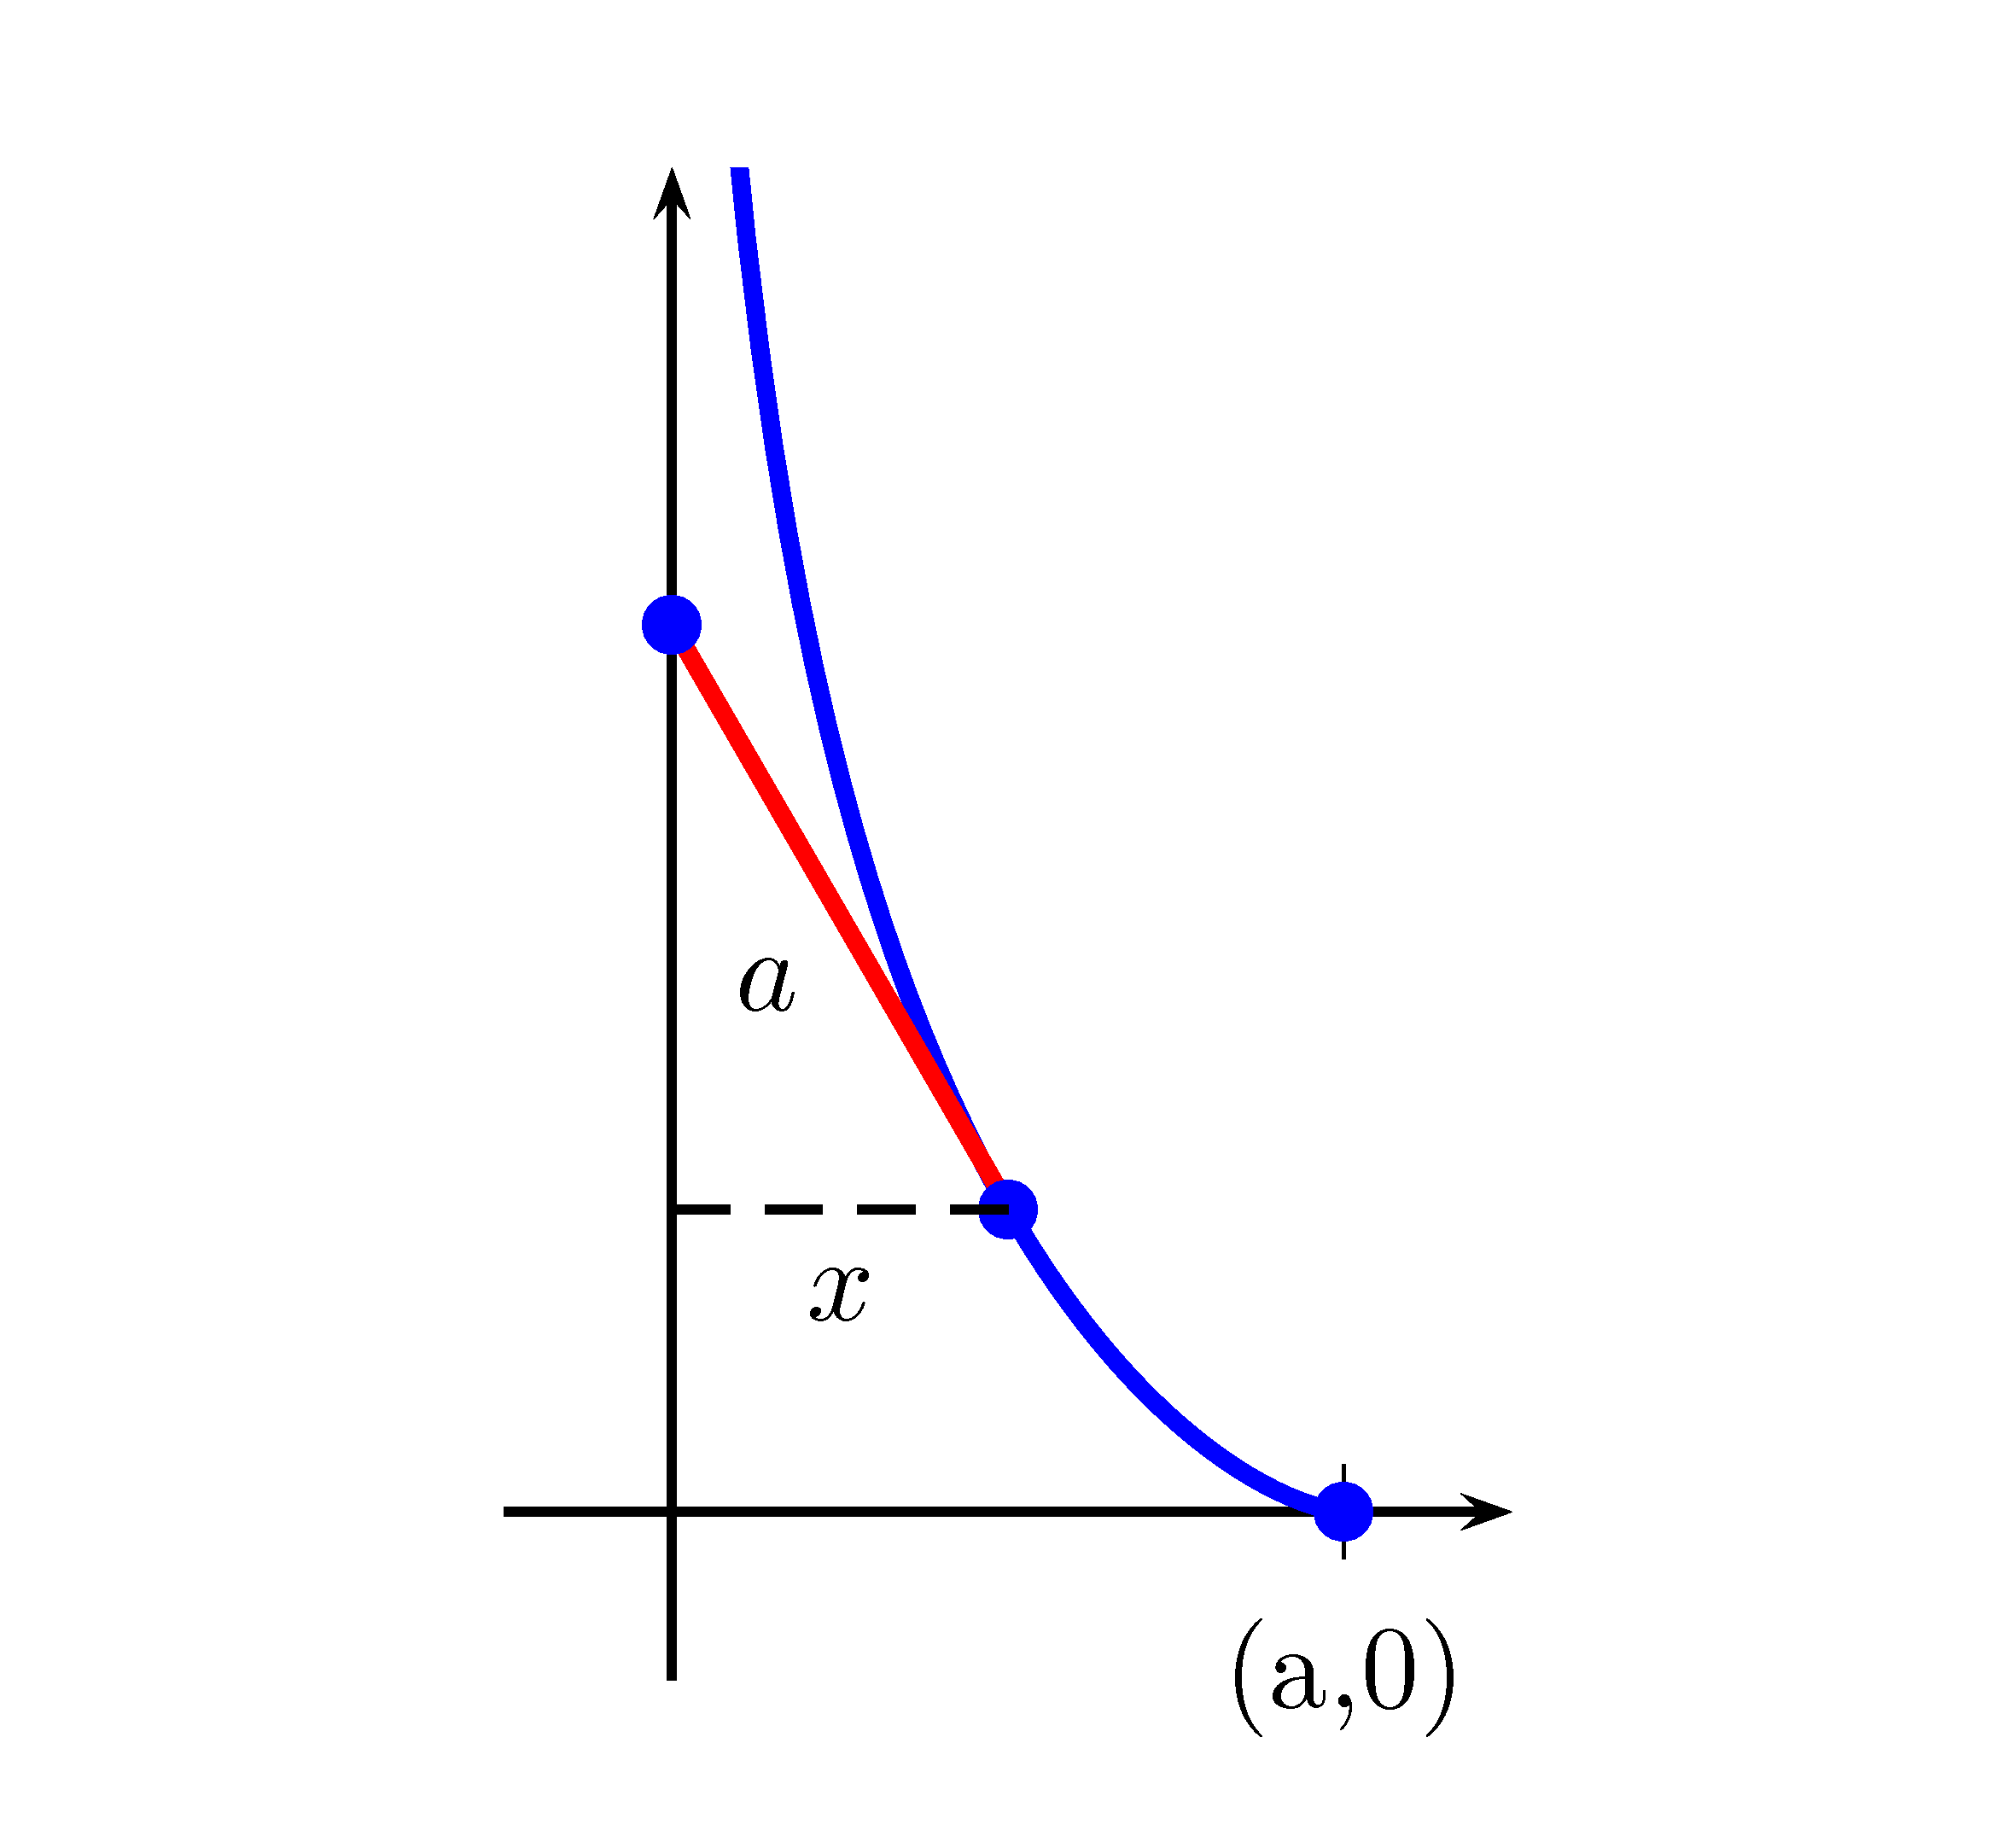
\includegraphics[width=0.75\linewidth]{resources/images/latex/tractrice} \end{center}
\vspace*{10cm}

\BeginKnitrBlock{example}
\protect\hypertarget{exm:unnamed-chunk-58}{}{\label{exm:unnamed-chunk-58}
}Trouvez les trajectoires orthogonales de la famille \(x=ky^2\).
\EndKnitrBlock{example}
\vspace*{8cm}

\BeginKnitrBlock{example}
\protect\hypertarget{exm:unnamed-chunk-59}{}{\label{exm:unnamed-chunk-59}
}Trouvez les trajectoires orthogonales de la famille \(y=ke^x\).
\EndKnitrBlock{example}
\vspace*{8cm}

\BeginKnitrBlock{example}
\protect\hypertarget{exm:parachutiste}{}{\label{exm:parachutiste} }Soit un
parachutiste qui tombe sous l'effet de la gravité avec une résistance de
l'air proportionnelle à sa vitesse. L'équation différentielle de cette
situation est : \(\dfrac{dv}{dt}+\dfrac{kv}{m}=g\) où \(m\), \(g\) et
\(k\) sont des constantes positives. Trouvez la solution de l'équation
différentielle précédente.
\EndKnitrBlock{example}
\vspace*{8cm}

\BeginKnitrBlock{example}
\protect\hypertarget{exm:unnamed-chunk-60}{}{\label{exm:unnamed-chunk-60}
}La loi de refroidissement de Newton dit que le taux de variation de la
température \(T\) d'un objet est proportionnel à la différence entre la
température de cet objet et la température ambiante (notée \(T_A\)).
Trouvez l'équation différentielle décrivant le phénomène et trouvez
\(T\) en fonction du temps.
\EndKnitrBlock{example}
\vspace*{8cm}

\hypertarget{les-equations-differentielles-lineaires}{%
\section{Les équations différentielles
linéaires}\label{les-equations-differentielles-lineaires}}

\BeginKnitrBlock{definition}[Équation différentielle linéaire]
\protect\hypertarget{def:unnamed-chunk-61}{}{\label{def:unnamed-chunk-61}
\iffalse (Équation différentielle linéaire) \fi{} }Une \textbf{équation
différentielle linéaire} est de la forme: \begin{align*}
\dfrac{dy}{dt}+P(t)y=Q(t)
\end{align*} où \(P(t)\) et \(Q(t)\) sont des fonctions qui ne doivent
dépendre que de la variable indépendante.
\EndKnitrBlock{definition}

\BeginKnitrBlock{example}
\protect\hypertarget{exm:unnamed-chunk-62}{}{\label{exm:unnamed-chunk-62}
}Voici quelques exemples d'équations différentielles linéaires:

\begin{itemize}
\tightlist
\item
  \(y'+t^2y=t^3\)
\item
  \(x^3y'-x^4y=1\) (Aprés division par \(x^2\))
\item
  \(y'=y\)
\end{itemize}
\EndKnitrBlock{example}

Pour être en mesure de résoudre ce type d'équations différentielles,
nous devrons tout d'abord utiliser une astuce.

Posons \(\mu(t)\) une fonction inconnue. Nous avons donc: \begin{align*}
\dfrac{d}{dt}[\mu y] &= \mu\dfrac{dy}{dt}+y\dfrac{d\mu}{dt} \\
&= \mu\left(Q(t)-P(t)y\right) + y\dfrac{d\mu}{dt} \qquad \text{car EDO linéaire}\\
&= \mu Q(t)-\mu P(t)y +y\dfrac{d\mu}{dt} \\
&= \mu Q(t)+y\left(\underbrace{\dfrac{d\mu}{dt}-\mu P(t)}_{\text{posons égal à 0}}\right)
\end{align*}

Ainsi: \begin{align*}
\dfrac{d}{dt}[\mu y] &= \mu Q(t) \\
\mu y &= \int \mu Q(t) \ dt\\
y &= \dfrac{1}{\mu} \int \mu Q(t) \ dt
\end{align*}

Pour pouvoir résoudre l'intégrale précédente, nous avons besoin de
connaître \(\mu\) et nous savons que: \begin{align*}
\dfrac{d\mu}{dt}-\mu P(t) &= 0 \\
\dfrac{d\mu}{dt} &= \mu P(t) \\
\int\dfrac{1}{\mu}d\mu &= \int P(t)dt \\
\ln |\mu| &= \int P(t)dt \\
\mu &= e^{\int P(t)dt}
\end{align*}

Pour résoudre une équation différentielle linéaire, il faut donc:

\begin{enumerate}
\def\labelenumi{\arabic{enumi}.}
\tightlist
\item
  Trouver \(\mu\): \(\mu = e^{\int P(t)dt}\)
\item
  Trouver \(y\): \(y = \dfrac{1}{\mu} \int \mu Q(t) \ dt\)
\end{enumerate}

\BeginKnitrBlock{example}
\protect\hypertarget{exm:unnamed-chunk-63}{}{\label{exm:unnamed-chunk-63}
}Trouvez la solution générale de \(y'+3\dfrac{y}{t}=1\).
\EndKnitrBlock{example}
\vspace*{8cm}

\BeginKnitrBlock{example}
\protect\hypertarget{exm:unnamed-chunk-64}{}{\label{exm:unnamed-chunk-64}
}Trouvez la solution générale de \(x^2y'+xy=1\) où \(x>0\) et
\(y(1)=2\).
\EndKnitrBlock{example}
\vspace*{8cm}

\BeginKnitrBlock{example}
\protect\hypertarget{exm:unnamed-chunk-65}{}{\label{exm:unnamed-chunk-65}
}Trouvez la solution générale de \(ty'+2y=t^2-t+1\).
\EndKnitrBlock{example}
\vspace*{8cm}

\BeginKnitrBlock{example}
\protect\hypertarget{exm:unnamed-chunk-66}{}{\label{exm:unnamed-chunk-66}
}Trouvez la solution générale de
\(\cos(x)y'+\sin(x)y=2\cos(x)^3\sin(x)-1\).
\EndKnitrBlock{example}
\vspace*{8cm}

\BeginKnitrBlock{example}
\protect\hypertarget{exm:unnamed-chunk-67}{}{\label{exm:unnamed-chunk-67}
}Résolvez l'équation différentielle du parachutiste, comme vu à
l'exemple \ref{exm:parachutiste}, en utilisant les équations
différentielles linéaires. L'équation différentielle est donnée par :
\(\dfrac{dv}{dt}+\dfrac{kv}{m}=g\).
\EndKnitrBlock{example}
\vspace*{8cm}

\hypertarget{problemes-de-melange}{%
\subsection{Problèmes de mélange}\label{problemes-de-melange}}

Dans des problèmes de mélange, nous cherchons \(Q(t)\) qui représente la
quantité d'une substance en fonction du temps. L'équation différentielle
de base de ce genre de problèmes est:

\begin{quote}
Taux de variation de \(Q(t)\) = Taux d'entrée de \(Q(t)\) - Taux de
sortie de \(Q(t)\)
\end{quote}

\BeginKnitrBlock{example}
\protect\hypertarget{exm:unnamed-chunk-68}{}{\label{exm:unnamed-chunk-68}
}Une cuve contient 10 L d'eau salée dans laquelle 2 kg de sel sont
dissout. De l'eau salée contenant 1 kg de sel par litre entre dans la
cuve à un débit constant de 3 L/min, et l'eau mélangée est vidée à un
taux de 4 L/min. Trouvez la quantité de sel en fonction du temps
\(Q(t)\).
\EndKnitrBlock{example}
\vspace*{10cm}

\BeginKnitrBlock{example}
\protect\hypertarget{exm:unnamed-chunk-69}{}{\label{exm:unnamed-chunk-69}
}Une cuve contient 40 L d'eau pure. De la saumure avec 3 kg de sel par
litre entre dans la cuve à un débit constant de 2 L/min, et la mixture
mélangée s'écoule à un débit constant de 3 L/min.

\begin{enumerate}
\def\labelenumi{\alph{enumi})}
\tightlist
\item
  Trouvez la quantité de sel en fonction du temps \(Q(t)\).
\item
  Quelle est la quantité de sel lorsqu'il reste 20 L dans la cuve?
\end{enumerate}
\EndKnitrBlock{example}
\vspace*{10cm}

\hypertarget{inverser-la-derivee}{%
\subsection{Inverser la dérivée}\label{inverser-la-derivee}}

Pour obtenir une équation différentielle linéaire, il faut parfois
étudier l'inverse de votre dérivée.

\begin{quote}
Plutôt que d'étudier \(\dfrac{dy}{dx}\), nous pouvons étudier
\(\dfrac{dx}{dy}\).
\end{quote}

\BeginKnitrBlock{example}
\protect\hypertarget{exm:unnamed-chunk-70}{}{\label{exm:unnamed-chunk-70}
}Trouvez la solution de l'équation différentielle
\((e^y-2xy)\dfrac{dy}{dx}=y^2\).
\EndKnitrBlock{example}
\vspace*{8cm}

\BeginKnitrBlock{example}
\protect\hypertarget{exm:unnamed-chunk-71}{}{\label{exm:unnamed-chunk-71}
}Trouvez les familles de courbes orthogonales à \(y^2=ce^x+x+1\) où
\(c\in\mathbb{R}\).
\EndKnitrBlock{example}
\vspace*{8cm}

\hypertarget{les-equations-differentielles-a-coefficients-constants-dordre-2}{%
\section{Les équations différentielles à coefficients constants d'ordre
2}\label{les-equations-differentielles-a-coefficients-constants-dordre-2}}

\hypertarget{quelques-rappels-concernant-les-nombres-complexes}{%
\subsection{Quelques rappels concernant les nombres
complexes}\label{quelques-rappels-concernant-les-nombres-complexes}}

\BeginKnitrBlock{definition}[Nombre complexe]
\protect\hypertarget{def:unnamed-chunk-72}{}{\label{def:unnamed-chunk-72}
\iffalse (Nombre complexe) \fi{} }Un nombre complexe \(z\) s'écrit sous
la forme \(z=a+bi\), où \(a,b \in \mathbb{R}\) et tel que \(i^2=-1\).

Nous disons que \(a\) est la partie réelle de \(z\) et \(b\) est la
partie imaginaire de \(z\).

L'ensemble des nombres complexes est noté \(\mathbb{C}\).

Nous pouvons également écrire \(z\) sous une form dite polaire qui est
\(z=r(\cos(\theta)+i\sin(\theta))\), où \(r=\sqrt{a^2+b^2}\) et
\(\theta=\text{Arctan}\left(\dfrac{b}{a}\right)\).
\EndKnitrBlock{definition}

La figure \ref{fig:nombrescomplexes} permet de représenter un nombre
complexe de façon géométrique.

\begin{figure}

{\centering 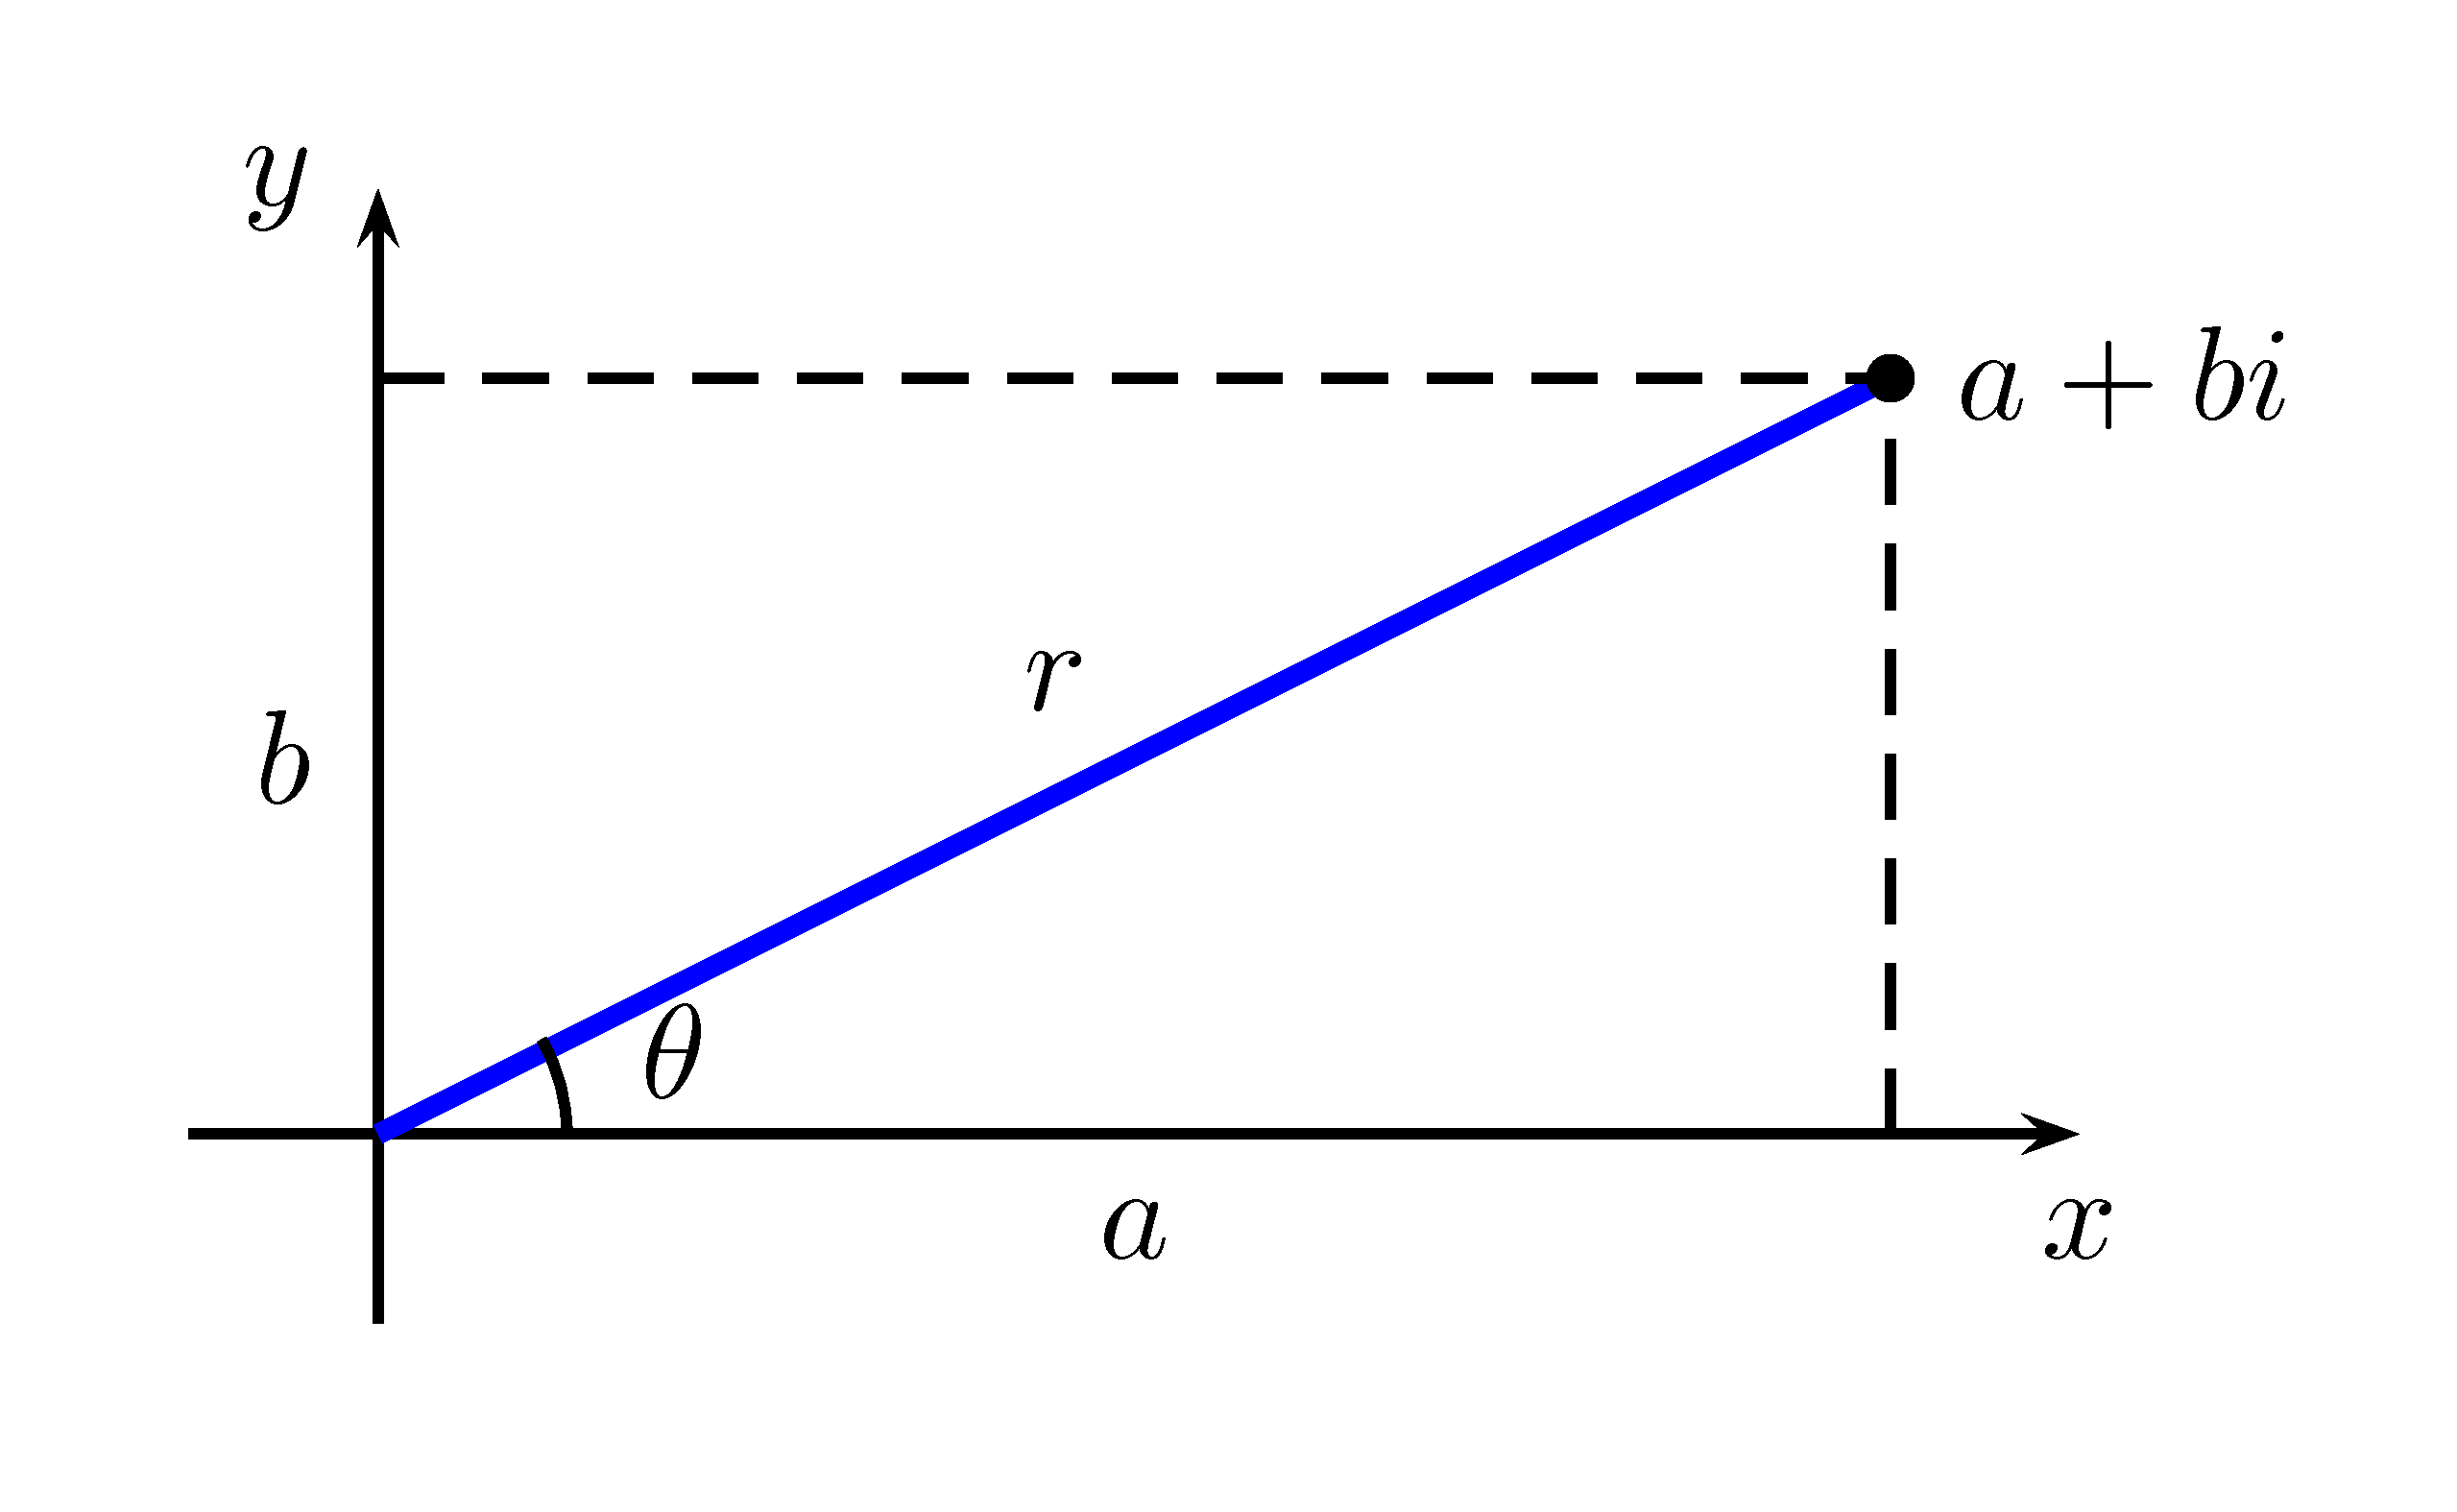
\includegraphics[width=0.5\linewidth]{resources/images/latex/nombrescomplexes} 

}

\caption{Représentation d'un nombre complexe}\label{fig:nombrescomplexes}
\end{figure}

\BeginKnitrBlock{theorem}[L'identité d'Euler]
\protect\hypertarget{thm:identite-euler}{}{\label{thm:identite-euler}
\iffalse (L'identité d'Euler) \fi{} }Soit le nombre complexe écrit sous
la forme \(z=r(\cos(\theta)+i\sin(\theta))\). Alors ce nombre peut
s'écrire de la manière suivante: \(z=re^{i\theta}\).
\EndKnitrBlock{theorem}

\BeginKnitrBlock{proof}
\iffalse{} {Preuve. } \fi{}La démonstration est laissée à l'étudiante ou
l'étudiant. \textbf{Astuce}: Il faut utiliser les séries de MacLaurin de
\(e^x\), \(\sin(x)\) et \(\cos(x)\).
\EndKnitrBlock{proof}

\BeginKnitrBlock{corollary}
\protect\hypertarget{cor:sin-cos-ei}{}{\label{cor:sin-cos-ei} }Nous avons:
\begin{align*}
\cos(\theta) &= \dfrac{e^{i\theta}+e^{-i\theta}}{2} \\
\sin(\theta) &= \dfrac{e^{i\theta}-e^{-i\theta}}{2i}
\end{align*}
\EndKnitrBlock{corollary}

\BeginKnitrBlock{proof}
\iffalse{} {Preuve. } \fi{}Pour démontrer ce résultat, nous utiliserons
le théorème \ref{thm:identite-euler}. Nous avons: \begin{align}
e^{i\theta} &= \cos(\theta)+i\sin(\theta)\label{eq:eplus} \\
e^{-i\theta} &= \cos(-\theta)+i\sin(-\theta) \notag \\
&= \cos(\theta)-i\sin(\theta)\label{eq:emoins}
\end{align}

Si nous additions les équations \eqref{eq:eplus} et \eqref{eq:emoins}:
\begin{align*}
e^{i\theta}+e^{-i\theta} &= \cos(\theta)+i\sin(\theta)+\cos(\theta)-i\sin(\theta) \\
&= 2\cos(\theta) \\
\cos(\theta) &= \dfrac{e^{i\theta}+e^{-i\theta}}{2}
\end{align*}

Si nous faisons la différence entre les équations \eqref{eq:eplus} et
\eqref{eq:emoins}: \begin{align*}
e^{i\theta}-e^{-i\theta} &= \cos(\theta)+i\sin(\theta)-(\cos(\theta)-i\sin(\theta)) \\
&= 2i\sin(\theta) \\
\sin(\theta) &= \dfrac{e^{i\theta}-e^{-i\theta}}{2i}
\end{align*}
\EndKnitrBlock{proof}

\hypertarget{les-equations-differentielles-homogenes-a-coefficients-constants-dordre-2}{%
\subsection{Les équations différentielles homogènes à coefficients
constants d'ordre
2}\label{les-equations-differentielles-homogenes-a-coefficients-constants-dordre-2}}

\BeginKnitrBlock{definition}[Équation différentielle homogène à coefficients constants d'ordre 2]
\protect\hypertarget{def:unnamed-chunk-75}{}{\label{def:unnamed-chunk-75}
\iffalse (Équation différentielle homogène à coefficients constants
d'ordre 2) \fi{} }Une \textbf{équation différentielle homogène à
coefficients constants d'ordre 2} est une équation différentielle de la
forme: \begin{align}
a\dfrac{d^2y}{dx^2}+b\dfrac{dy}{dx}+cy &= 0 \label{eq:homogene2}
\end{align} où \(a,b,c \in \mathbb{R}\) et \(a\neq 0\).
\EndKnitrBlock{definition}

\begin{quote}
Le terme \emph{homogène} indique que le membre de droite de l'équation
\eqref{eq:homogene2} est nul. Nous traiterons le cas à la section
\ref{non-homogene-2}.
\end{quote}

Avant de résoudre ce type d'équations différentielles, la prochaine
proposition sera cruciale.

\BeginKnitrBlock{proposition}
\protect\hypertarget{prp:combinaison-lineaire-solution}{}{\label{prp:combinaison-lineaire-solution}
}Si \(y_1(x)\) et \(y_2(x)\) sont deux solutions de l'équation
\eqref{eq:homogene2}, alors \(y(x)=C_1y_1(x)+C_2y_2(x)\), où
\(C_1,C_2\in\mathbb{R}\), est aussi une solution de l'équation
\eqref{eq:homogene2}.
\EndKnitrBlock{proposition}

\BeginKnitrBlock{proof}
\iffalse{} {Preuve. } \fi{}Nous avons que: \begin{align*}
ay_1''+by_1'+cy_1 &= 0 \\
ay_2''+by_2'+cy_2 &= 0
\end{align*} car \(y_1\) et \(y_2\) sont des solutions de
\eqref{eq:homogene2}. Nous avons que: \begin{align*}
y &= C_1y_1+C_2y_2 \\
y' &= C_1y_1'+C_2y_2' \\
y'' &= C_1y_1''+C_2y_2'' \\
\end{align*} Ainsi: \begin{align*}
ay''+by'+cy &= a(C_1y_1''+C_2y_2'')+b(C_1y_1'+C_2y_2')+c(C_1y_1+C_2y_2) \\
&= C_1\underbrace{(ay_1''+by_1'+cy_1)}_{=\ 0}+C_2\underbrace{(ay_2''+by_2'+cy_2)}_{=\ 0} \\
&= 0
\end{align*}
\EndKnitrBlock{proof}

\begin{quote}
Une combinaison linéaire de solutions est aussi une solution.
\end{quote}

Nous pouvons maintenant résoudre l'équation \eqref{eq:homogene2} en
supposant que la solution est de la forme \(y=e^{rx}\), où \(r\) est une
constante qu'il nous reste à déterminer.

\begin{quote}
Pour résoudre une équation différentielle homogène d'ordre 2 à
coefficients constants, il faut toujours poser la solution \(y=e^{rx}\).
\end{quote}

Nous avons donc: \begin{align*}
y &= e^{rx} \\
y' &= re^{rx} \\
y'' &= r^2e^{rx}
\end{align*}

Nous substituons ces résultats dans l'équation \eqref{eq:homogene2}:
\begin{align}
a\dfrac{d^2y}{dx^2}+b\dfrac{dy}{dx}+cy &= 0 \notag \\
ar^2e^{rx}+bre^{rx}+ce^{rx} &= 0 \notag \\
e^{rx}(ar^2+br+c) &= 0 \notag \\
ar^2+br+c &= 0\label{eq:quadratique}
\end{align}

L'équation \eqref{eq:quadratique} se nomme polynôme caractéristique de
l'équation \eqref{eq:homogene2}. Déterminer les valeurs de \(r\) revient à
trouver les racines du polynôme caractéristique et donc: \begin{align*}
r_{1,2} &= \dfrac{-b\pm\sqrt{b^2-4ac}}{2a}
\end{align*} Nous devrons étudier trois cas distincts qui dépendent du
discriminant \(b^2-4ac\).

\hypertarget{cas-1-b2-4ac0}{%
\subsubsection{\texorpdfstring{Cas 1:
\(b^2-4ac>0\)}{Cas 1: b\^{}2-4ac\textgreater{}0}}\label{cas-1-b2-4ac0}}

Dans ce cas, le polynôme caractéristique fournit deux valeurs de \(r\)
\textbf{réelles}, que nous notons \(r_1\) et \(r_2\). Nous avons donc
\(y_1(x)=e^{r_1x}\) qui est une solution de \eqref{eq:homogene2} et
également \(y_2=e^{r_2x}\). Par la proposition
\ref{prp:combinaison-lineaire-solution}, nous obtenons la solution
générale: \begin{align*}
y(x) &= C_1e^{r_1x}+C_2e^{r_2x}
\end{align*} où \(C_1,C_2\in\mathbb{R}\).

\BeginKnitrBlock{example}
\protect\hypertarget{exm:unnamed-chunk-77}{}{\label{exm:unnamed-chunk-77}
}Résolvez l'équation différentielle \(y''+y'-6y=0\) avec comme
conditions initiales \(y(0)=0\) et \(y'(0)=1\).
\EndKnitrBlock{example}
\vspace*{10cm}

\hypertarget{cas-2-b2-4ac0}{%
\subsubsection{\texorpdfstring{Cas 2:
\(b^2-4ac<0\)}{Cas 2: b\^{}2-4ac\textless{}0}}\label{cas-2-b2-4ac0}}

Dans ce cas, le polynôme caractéristique fournit deux valeurs de \(r\)
\textbf{complexes}. Posons \(\gamma=-\dfrac{b}{2a}\) et
\(\omega=\dfrac{\sqrt{4ac-b^2}}{2a}\) ce qui implique que
\(r_1=\gamma+\omega i\) et \(r_2=\gamma -\omega i\). Nous avons donc
deux solutions à l'équation \eqref{eq:homogene2}, soit
\(y_1=e^{r_1x}=e^{(\gamma+\omega i)x}\) et
\(y_2=e^{r_2x}=e^{(\gamma-\omega i)x}\).

Puisque les solutions précédentes sont complexes, nous allons utiliser
la proposition \ref{prp:combinaison-lineaire-solution} et le corollaire
\ref{cor:sin-cos-ei} pour créer deux nouvelles solutions réelles:
\begin{align*}
y_3(x) &= \dfrac{y_1(x)+y_2(x)}{2} \\
&= \dfrac{e^{(\gamma+\omega i)x}+e^{(\gamma-\omega i)x}}{2} \\
&= e^{\gamma x}\left( \dfrac{e^{\omega i x}+e^{-\omega i x}}{2} \right) \\
&= e^{\gamma x}\cos(\omega x) \\
y_4(x) &= \dfrac{y_1(x)-y_2(x)}{2i} \\
&= \dfrac{e^{(\gamma+\omega i)x}-e^{(\gamma-\omega i)x}}{2i} \\
&= e^{\gamma x}\left( \dfrac{e^{\omega i x}-e^{-\omega i x}}{2i} \right) \\
&= e^{\gamma x}\sin(\omega x)
\end{align*}

D'où la solution générale de l'équation \eqref{eq:homogene2} est:
\begin{align*}
y(x) &= e^{\gamma x}\left( C_1\cos(\omega x)+C_2\sin(\omega x) \right)
\end{align*}

\BeginKnitrBlock{example}
\protect\hypertarget{exm:unnamed-chunk-78}{}{\label{exm:unnamed-chunk-78}
}Trouvez la solution de l'équation différentielle \(y''+2y'+10y=0\)
ayant comme conditions initiales \(y(0)=0\) et \(y'(0)=3\).
\EndKnitrBlock{example}
\vspace*{10cm}

\hypertarget{cas-3-b2-4ac0}{%
\subsubsection{\texorpdfstring{Cas 3:
\(b^2-4ac=0\)}{Cas 3: b\^{}2-4ac=0}}\label{cas-3-b2-4ac0}}

Dans ce cas, nous n'obtenons qu'une seule valeur de
\(r=-\dfrac{b}{2a}\). Puisque nous n'avons qu'une seule solution, nous
devons en trouver une autre pour être en mesure de construire une
combinaison linéaire. Nous allons démontrer que \(y_2(x)=xe^{rx}\) est
aussi une solution de l'équation différentielle \eqref{eq:homogene2}.
\BeginKnitrBlock{proof}
\iffalse{} {Preuve. } \fi{}\begin{align*}
y_2 &= xe^{rx} \\
y_2' &= e^{rx}+rxe^{rx} \\
y_2'' &= re^{rx}+re^{rx}+r^2xe^{rx}
\end{align*} Et donc: \begin{align*}
ay'' +by' +cy &= 0 \\
a(2re^{rx}+r^2xe^{rx})+b(e^{rx}+rxe^{rx})+c(xe^{rx}) &= 0 \\
e^{rx}(2ar+ar^2x+b+brx+cx) &= 0 \\
e^{rx}(\underbrace{(ar^2+br+c)}_{=0}x+\underbrace{(2ar+b)}_{=0}) &= 0 
\end{align*}
\EndKnitrBlock{proof}

La solution générale est donc de la forme: \begin{align*}
y(x) &= C_1e^{rx}+C_2xe^{rx}
\end{align*}

\BeginKnitrBlock{example}
\protect\hypertarget{exm:unnamed-chunk-80}{}{\label{exm:unnamed-chunk-80}
}Trouvez la solution de l'équation différentielle \(y''+2y'+y=0\).
\EndKnitrBlock{example}
\vspace*{5cm}

\BeginKnitrBlock{example}
\protect\hypertarget{exm:unnamed-chunk-81}{}{\label{exm:unnamed-chunk-81}
}Trouvez les solutions des équations différentielles suivantes:

\begin{enumerate}
\def\labelenumi{\alph{enumi})}
\tightlist
\item
  \(y''-9y'+20y=0\)
\item
  \(2y''-4y'+8y=0\)
\item
  \(y''+6y'+9=0\)
\end{enumerate}
\EndKnitrBlock{example}
\vspace*{20cm}

\hypertarget{non-homogene-2}{%
\subsection{Les équations différentielles non homogènes à coefficients
constants d'ordre 2}\label{non-homogene-2}}

\BeginKnitrBlock{definition}[Équation différentielle non homogène à coefficients constants d'ordre 2]
\protect\hypertarget{def:unnamed-chunk-82}{}{\label{def:unnamed-chunk-82}
\iffalse (Équation différentielle non homogène à coefficients constants
d'ordre 2) \fi{} }Une \textbf{équation différentielle non homogène à
coefficients constants d'ordre 2} est une équation différentielle de la
forme: \begin{align}
a\dfrac{d^2y}{dx^2}+b\dfrac{dy}{dx}+cy &= F(x) \label{eq:nonhomogene2}
\end{align} où \(a,b,c \in \mathbb{R}\) et \(a\neq 0\). De plus \(F(x)\)
est une fonction qui ne dépend que de la variable indépendante.
\EndKnitrBlock{definition}

Pour résoudre ce type d'équations différentielles, nous aurons besoin du
théorème suivant:

\BeginKnitrBlock{theorem}
\protect\hypertarget{thm:unnamed-chunk-83}{}{\label{thm:unnamed-chunk-83}
}Soit une équation différentielle de la forme: \begin{align*}
a\dfrac{d^2y}{dx^2}+b\dfrac{dy}{dx}+cy &= F(x)
\end{align*} La solution de cette équation différentielle est de la
forme: \begin{align*}
y(x) &= C_1y_1(x)+C_2y_2(x)+y_p
\end{align*} où \(y_1\) et \(y_2\) sont les solutions de l'équation
homogène associée à l'équation \eqref{eq:nonhomogene2}, c'est-à-dire:
\begin{align*}
a\dfrac{d^2y}{dx^2}+b\dfrac{dy}{dx}+cy &= 0
\end{align*} et \(y_p\) est une solution particulière de l'équation non
homogène.
\EndKnitrBlock{theorem}

\BeginKnitrBlock{proof}
\iffalse{} {Preuve. } \fi{}La démonstration est laissée à l'étudiante ou
à l'étudiant.
\EndKnitrBlock{proof}

Nous verrons deux méthodes pour trouver \(y_p\).

\hypertarget{la-methode-des-coefficients-indetermines}{%
\subsubsection{La méthode des coefficients
indéterminés}\label{la-methode-des-coefficients-indetermines}}

Cette méthode consiste à étudier la nature de la fonction \(F(x)\) et à
supposer que \(y_p\) est de même nature. La table
\ref{tab:coeff-indetermines} montre la forme de la solution particulière
\(y_p\) selon la nature de \(F(x)\).

\begin{longtable}[]{@{}cc@{}}
\caption{\label{tab:coeff-indetermines} Les diverses formes de coefficients
indéterminés.}\tabularnewline
\toprule
\begin{minipage}[b]{0.55\columnwidth}\centering
Forme de \(F(x)\)\strut
\end{minipage} & \begin{minipage}[b]{0.39\columnwidth}\centering
Forme de \(y_p\)\strut
\end{minipage}\tabularnewline
\midrule
\endfirsthead
\toprule
\begin{minipage}[b]{0.55\columnwidth}\centering
Forme de \(F(x)\)\strut
\end{minipage} & \begin{minipage}[b]{0.39\columnwidth}\centering
Forme de \(y_p\)\strut
\end{minipage}\tabularnewline
\midrule
\endhead
\begin{minipage}[t]{0.55\columnwidth}\centering
Polynôme de degré \(n\)\strut
\end{minipage} & \begin{minipage}[t]{0.39\columnwidth}\centering
\(y_p=a_nx^n+a_{n-1}x^{n-1}+\ldots+a_x+a_0\)\strut
\end{minipage}\tabularnewline
\begin{minipage}[t]{0.55\columnwidth}\centering
\(F(x)\) possède un \(\sin(\omega x)\) et/ou un \(\cos(\omega x)\)\strut
\end{minipage} & \begin{minipage}[t]{0.39\columnwidth}\centering
\(y_p=A\cos(\omega x)+B\sin(\omega x)\)\strut
\end{minipage}\tabularnewline
\begin{minipage}[t]{0.55\columnwidth}\centering
\(F(x)\) possède une exponentielle \(e^{\alpha x}\)\strut
\end{minipage} & \begin{minipage}[t]{0.39\columnwidth}\centering
\(y_p=A^{\alpha x}\)\strut
\end{minipage}\tabularnewline
\bottomrule
\end{longtable}

\BeginKnitrBlock{example}
\protect\hypertarget{exm:unnamed-chunk-85}{}{\label{exm:unnamed-chunk-85}
}Trouvez la solution générale de l'équation différentielle
\(y''+y'-6y=3x^2\).
\EndKnitrBlock{example}
\vspace*{10cm}

\BeginKnitrBlock{example}
\protect\hypertarget{exm:unnamed-chunk-86}{}{\label{exm:unnamed-chunk-86}
}Trouvez la solution générale de l'équation différentielle
\(y''+y'-6y=e^{4x}+\cos(3x)\).
\EndKnitrBlock{example}
\vspace*{10cm}

\BeginKnitrBlock{example}
\protect\hypertarget{exm:unnamed-chunk-87}{}{\label{exm:unnamed-chunk-87}
}Trouvez la solution générale de l'équation différentielle
\(y''+2y'+10y=\cos(2t)\) avec les conditions intiales
\(y(0)=-\frac{1}{2}\) et \(y'(0)=4\).
\EndKnitrBlock{example}
\vspace*{15cm}

\hypertarget{la-methode-de-variation-des-parametres-ou-methode-de-lagrange}{%
\subsubsection{La méthode de variation des paramètres (ou méthode de
Lagrange)}\label{la-methode-de-variation-des-parametres-ou-methode-de-lagrange}}

La méthode de variation des paramètres est souvent plus longue à
utiliser que la méthode des coefficients indéterminés, par contre, elle
est valide pour tous les types de fonctions \(F(x)\).

Nous débutons en trouvant les solutions \(y_1\) et \(y_2\) de l'équation
différentielle homogène associée à l'équation: \begin{align*}
ay''+by'+cy=F(x)
\end{align*}

Supposons que la solution est de la forme : \begin{align*}
y(x) &= \mu_1(x)y_1(x)+\mu_2(x)y_2(x)
\end{align*} Afin d'alléger la notation, nous omettrons la dépendance en
\(x\). Nous cherchons donc \(\mu_1\) et \(\mu_2\). Avant de substituer
dans l'équation différentielle, nous allons trouver les dérivées
successives de \(y\). \begin{align*}
y' &= \mu_1y_1'+\mu_1'y_1+\mu_2'y_2+\mu_2y_2'
\end{align*} Nous allons maintenant faire la supposition que
\(\mu_1'y_1+\mu_2'y_2=0\) et donc: \begin{align*}
y' &= \mu_1y_1'+\mu_2y_2'
\end{align*} Trouvons maintenant la dérivée seconde: \begin{align*}
y' &= \mu_1'y_1'+\mu_1y_1''+\mu_2'y_2'+\mu_2y_2''
\end{align*} Nous avons donc: \begin{align*}
ay''+by'+cy &= F(x) \\
a(\mu_1'y_1'+\mu_1y_1''+\mu_2'y_2'+\mu_2y_2'')+b(\mu_1y_1'+\mu_2y_2')+c(\mu_1y_1+\mu_2y_2) &= F(x) \\
\mu_1\underbrace{(ay_1''+by_1'+cy_1)}_{=0}+\mu_2\underbrace{(ay_2''+by_2'+cy_2)}_{=0}+\mu_1'y_1'+\mu_2'y_2' &= F(x) \\
\mu_1'y_1'+\mu_2'y_2' &= F(x)
\end{align*} Ainsi, pour déterminer \(\mu_1\) et \(\mu_2\), nous avons
les deux équations suivantes: \begin{align*}
\mu_1'y_1+\mu_2'y_2 &= 0 \\
\mu_1'y_1'+\mu_2'y_2' &= F(x)
\end{align*} Nous pouvons utiliser la méthode de Cramer pour résoudre ce
système d'équations linéaires: \begin{align*}
\mu_1'&= \dfrac{
\begin{vmatrix}
0&y_2\\
F(x)&y_2'
\end{vmatrix}}{
\begin{vmatrix}
y_1 &y_2\\
y_1'&y_2'
\end{vmatrix}
}=-\dfrac{y_2F(x)}{W(y_1,y_2)}\\
\mu_2'&= \dfrac{
\begin{vmatrix}
y_1&0\\
y_1'&F(x)
\end{vmatrix}}{
\begin{vmatrix}
y_1 &y_2\\
y_1'&y_2'
\end{vmatrix}
}=\dfrac{y_1F(x)}{W(y_1,y_2)}
\end{align*}

\BeginKnitrBlock{definition}[Wronskien]
\protect\hypertarget{def:unnamed-chunk-88}{}{\label{def:unnamed-chunk-88}
\iffalse (Wronskien) \fi{} }Nous appelons le \textbf{Wronskien} de deux
fonctions \(y_1\) et \(y_2\), le résultat suivant: \begin{align*}
W(y_1,y_2)=\begin{vmatrix}
y_1 &y_2\\
y_1'&y_2'
\end{vmatrix}
\end{align*}
\EndKnitrBlock{definition}

\BeginKnitrBlock{remark}
\iffalse{} {Remarque. } \fi{}Le \textbf{Wronskien} n'est jamais égal à
zéro lorsque nous résolvons une équation différentielle car \(y_1\) et
\(y_2\) sont choisies pour être linéairement indépendantes.
\EndKnitrBlock{remark}

Nous pouvons maintenant trouver nos deux fonctions \(\mu_1\) et
\(\mu_2\): \begin{align*}
\mu_1&=-\int \dfrac{y_2(x)F(x)}{W(y_1,y_2)}dx\\
\mu_2&=\int \dfrac{y_1(x)F(x)}{W(y_1,y_2)}dx
\end{align*}

\BeginKnitrBlock{example}
\protect\hypertarget{exm:unnamed-chunk-90}{}{\label{exm:unnamed-chunk-90}
}Trouvez la solution particulière de l'équation différentielle
\(y''+y=\csc(x)\).
\EndKnitrBlock{example}
\vspace*{10cm}

\BeginKnitrBlock{example}
\protect\hypertarget{exm:unnamed-chunk-91}{}{\label{exm:unnamed-chunk-91}
}Trouvez les solutions des équations différentielles suivantes en
utilisant les deux méthodes:

\begin{itemize}
\tightlist
\item
  Méthode des coefficients indéterminés
\item
  Méthode de variation des paramètres
\end{itemize}

\begin{enumerate}
\def\labelenumi{\alph{enumi}.}
\tightlist
\item
  \(y''-2y'+y=2x\)
\item
  \(y''-y'-6y=e^{-x}\)
\end{enumerate}
\EndKnitrBlock{example}

\hypertarget{applications-des-equations-differentielles-du-deuxieme-ordre-a-coefficients-constants}{%
\section{Applications des équations différentielles du deuxième ordre à
coefficients
constants}\label{applications-des-equations-differentielles-du-deuxieme-ordre-a-coefficients-constants}}

Nous discuterons en particulier de l'oscillateur harmonique forcé.

\BeginKnitrBlock{example}[Oscillateur harmonique forcé]
\protect\hypertarget{exm:unnamed-chunk-92}{}{\label{exm:unnamed-chunk-92}
\iffalse (Oscillateur harmonique forcé) \fi{} }Soit un ressort de
constante \(k\) auquel nous attachons une masse \(M\). Si le frottement
est proportionnel à la vitesse de la masse et que celle-ci subit une
force périodique, nous pouvons décrire le mouvement avec l'équation
suivante: \begin{align*}
\dfrac{d^2x}{dt^2}+\dfrac{c}{M}\dfrac{dx}{dt}+\dfrac{k}{M}x &= \dfrac{F_0}{M}\cos(\omega t)
\end{align*} Nous pouvons réécrire l'équation précédente en introduisant
les variables \(b=\dfrac{c}{2M}\) et \(a=\sqrt{\dfrac{k}{M}}\):
\begin{align*}
\dfrac{d^2x}{dt^2}+2b\dfrac{dx}{dt}+a^2x &= \dfrac{F_0}{M}\cos(\omega t)
\end{align*} Ce changement nous simplifiera le travail.

\begin{enumerate}
\def\labelenumi{\alph{enumi}.}
\tightlist
\item
  Trouvez la solution homogène de l'équation différentielle.
\item
  Supposez que \(b=0\), c'est-à-dire qu'il n'y a pas de frottement.
  Trouvez la solution particulière dans le cas où \(a\neq \omega\).
  (Vous étudiez dans ce cas la situation des \textbf{battements}). Pour
  en savoir plus sur le phénomène de
  \href{https://fr.wikipedia.org/wiki/Battement_(physique)}{battements}.
\item
  Supposez que \(b=0\), c'est-à-dire qu'il n'y a pas de frottement.
  Trouvez la solution particulière dans le cas où \(a =\omega\). (Vous
  étudiez dans ce cas la situation de \textbf{résonnance}) Pour voir en
  action le phénomène de résonnance,
  \href{https://www.youtube.com/watch?v=j-zczJXSxnw}{Tacoma Narrows
  Bridge} .
\end{enumerate}
\EndKnitrBlock{example}

\hypertarget{geogebra-edo}{%
\section{GeoGebra}\label{geogebra-edo}}

\hypertarget{applet_container}{}

\newpage

\hypertarget{pages-supplementaires-1}{%
\section{Pages supplémentaires}\label{pages-supplementaires-1}}

Des pages blanches supplémentaires pour ajouter, potentiellement, de
nouveaux exemples et exercices.

\multido{\i=0+1}{5}{
\newpage
\mbox{}
}

\hypertarget{coordpolaires}{%
\chapter{Les coordonnées polaires}\label{coordpolaires}}

Vous trouverez à la section \ref{geogebra-polaire} une application
\href{https://www.geogebra.org/?lang=fr}{GeoGebra} vous permettant de
visualiser des courbes en coordonnées polaires. À noter que cette
application n'est disponible que dans la version en ligne de ce
document.

\hypertarget{introduction-2}{%
\section{Introduction}\label{introduction-2}}

Les coordonnées polaires sont un autre système pour décrire un point
\(P\) de \(\mathbb{R}^2\). Les coordonnées cartésiennes associent à
chaque point \(P\) un couple \((x,y)\). Les coordonnées polaires
consistent à décrire ce point \(P\) avec le couple \((r,\theta)\), où
\(r\) est la longueur du segment de droite reliant l'origine au point
\(P\) et \(\theta\) est l'angle entre ce segment de droite et l'axe des
\(x\) positifs. La figure \ref{fig:coordpolaires} représente ce type de
coordonnées.

\begin{figure}

{\centering 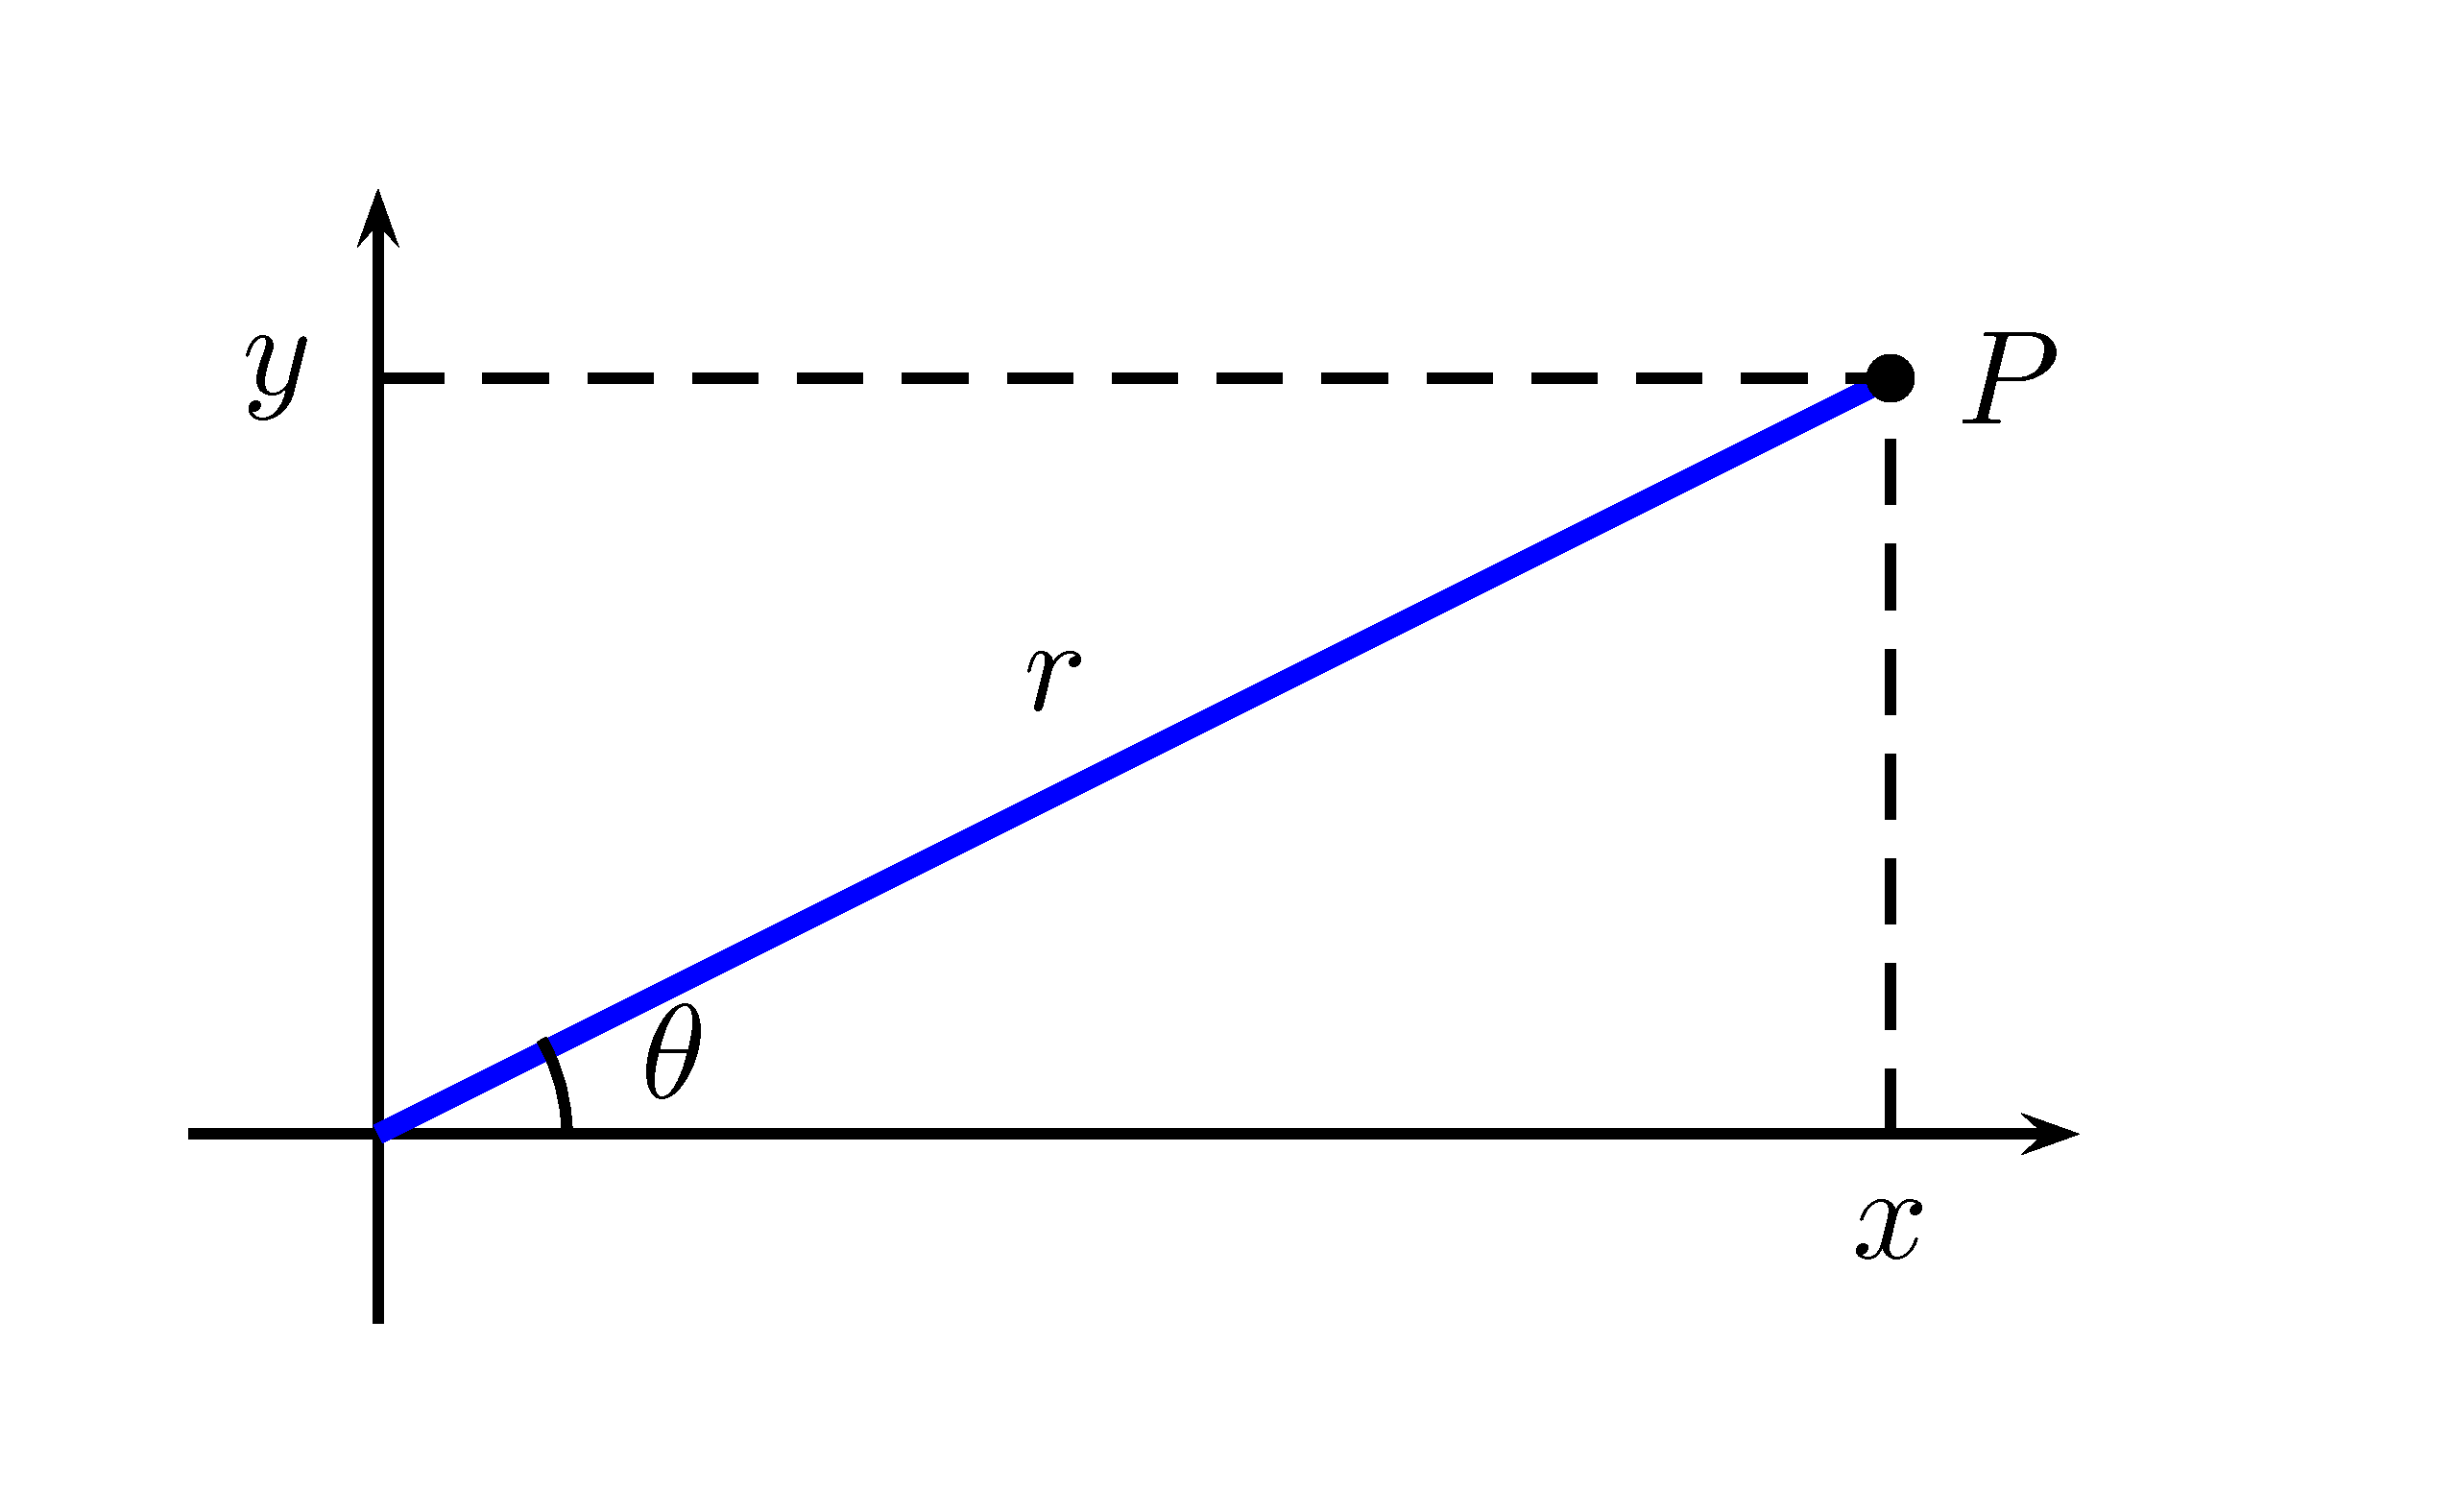
\includegraphics[width=0.5\linewidth]{resources/images/latex/coordpolaires} 

}

\caption{Coordonnées polaires d'un point $P$}\label{fig:coordpolaires}
\end{figure}

Il est primordial de pouvoir convertir les coordonnées cartésiennes à
des coordonnées polaires et vice-versa.

\BeginKnitrBlock{proposition}[Coordonnées cartésiennes à coordonnées polaires]
\protect\hypertarget{prp:unnamed-chunk-93}{}{\label{prp:unnamed-chunk-93}
\iffalse (Coordonnées cartésiennes à coordonnées polaires) \fi{} }Soit
un point \(P\) en coordonnées cartésiennes \((x,y)\). La conversion en
coordonnées polaires est: \begin{align*}
r &= \sqrt{x^2+y^2} \\
\theta &= \text{Arctan}\left(\dfrac{y}{x}\right)
\end{align*}
\EndKnitrBlock{proposition}

\BeginKnitrBlock{proposition}[Coordonnées polaires à coordonnées cartésiennes]
\protect\hypertarget{prp:unnamed-chunk-94}{}{\label{prp:unnamed-chunk-94}
\iffalse (Coordonnées polaires à coordonnées cartésiennes) \fi{} }Soit
un point \(P\) en coordonnées polaires \((r,\theta)\). La conversion en
coordonnées cartésiennes est: \begin{align*}
x &= r\cos(\theta) \\
y &= r\sin(\theta)
\end{align*}
\EndKnitrBlock{proposition}

\BeginKnitrBlock{remark}
\iffalse{} {Remarque. } \fi{}Voici quelques remarques:

\begin{enumerate}
\def\labelenumi{\arabic{enumi}.}
\tightlist
\item
  L'origine, c'est-à-dire le point \((0,0)\) en coordonnées
  cartésiennes, que l'on appelle pôle, peut s'écrire \((0,\theta)\), et
  ce, pour toutes les valeurs de \(\theta\) possibles. Ceci signifie
  qu'il n'existe pas de bijection\footnote{Une bijection est une
    fonction \(f\) allant d'un ensemble \(A\) à un ensemble \(B\), telle
    que pour tous les éléments de \(B\), on associe une seule valeur de
    \(A\).} entre les coordonnées cartésiennes et polaires. Par contre,
  si on enlève l'origine, il en existe une.
\item
  Lorsque l'on fixe \(\theta=\theta_0\), l'ensemble formé par
  \((r,\theta_0)\)est une demi-droite. En acceptant que \(r\) soit
  négatif, on obtient alors que \((r,\theta_0)\) forme une droite.
\item
  Si \(r>0\), alors \((-r,\theta_0)=(r,\theta_0+\pi)\).
\end{enumerate}
\EndKnitrBlock{remark}

\BeginKnitrBlock{example}
\protect\hypertarget{exm:unnamed-chunk-96}{}{\label{exm:unnamed-chunk-96}
}Écrivez les points suivants en coordonnées polaires:

\begin{enumerate}
\def\labelenumi{\alph{enumi}.}
\tightlist
\item
  \(P_1=(1,1)\)
\item
  \(P_2=(-\sqrt{3},1)\)
\item
  \(P_3=(0,-2)\)
\end{enumerate}
\EndKnitrBlock{example}
\vspace*{10cm}

\BeginKnitrBlock{example}
\protect\hypertarget{exm:unnamed-chunk-97}{}{\label{exm:unnamed-chunk-97}
}Écrivez les points suivants en coordonnées cartésiennes:

\begin{enumerate}
\def\labelenumi{\alph{enumi}.}
\tightlist
\item
  \((2,\pi/3)\)
\item
  \((3,3\pi/4)\)
\end{enumerate}
\EndKnitrBlock{example}
\vspace*{10cm}

\BeginKnitrBlock{example}
\protect\hypertarget{exm:unnamed-chunk-98}{}{\label{exm:unnamed-chunk-98}
}Écrivez l'équation de la perle de Sluze en coordonnées polaires, si
\(y^2=x(8-x)\).
\EndKnitrBlock{example}
\vspace*{6cm}

\hypertarget{le-graphique-dune-equation-polaire-rftheta}{%
\section{\texorpdfstring{Le graphique d'une équation polaire
\(r=f(\theta)\)}{Le graphique d'une équation polaire r=f(\textbackslash{}theta)}}\label{le-graphique-dune-equation-polaire-rftheta}}

Étudions maintenant comment représenter graphiquement des équations
polaires de la forme \(r=f(\theta)\). Nous généraliserons le tout pour
des équations implicites de la forme \(F(r,\theta)=0\).

\BeginKnitrBlock{example}
\protect\hypertarget{exm:unnamed-chunk-99}{}{\label{exm:unnamed-chunk-99}
}Dessinez la courbe \(r=K\) où \(K\) est une constante et \(K>0\).
\EndKnitrBlock{example}
\vspace*{5cm}

\BeginKnitrBlock{example}
\protect\hypertarget{exm:unnamed-chunk-100}{}{\label{exm:unnamed-chunk-100}
}Dessinez la courbe \(\theta=\dfrac{\pi}{4}\).
\EndKnitrBlock{example}
\vspace*{5cm}

Pour être en mesure de dessiner des relations en coordonnées polaires,
nous aurons besoin d'une grille polaire.

\BeginKnitrBlock{definition}[Grille polaire]
\protect\hypertarget{def:unnamed-chunk-101}{}{\label{def:unnamed-chunk-101}
\iffalse (Grille polaire) \fi{} }Une grille polaire est une grille où
nous traçons les courbes telles que \(r\) est constant, c'est-à-dire des
cercles centrés en \((0,0)\) et telles que \(\theta\) est constante,
c'est-à-dire les droites passant par l'origine et faisant un angle
\(\theta\) avec l'axe des \(x\).

Nous représentons habituellement les cercles de rayons \(1\) à \(5\) et
les droites d'angles \(\frac{\pi}{6}\) (\(30^{\circ}\)),
\(\frac{\pi}{4}\) (\(45^{\circ}\)) et \(\frac{\pi}{3}\)
(\(60^{\circ}\)).

Une grille polaire est représentée à la figure \ref{fig:grillepolaire}.
\EndKnitrBlock{definition}

\begin{figure}

{\centering 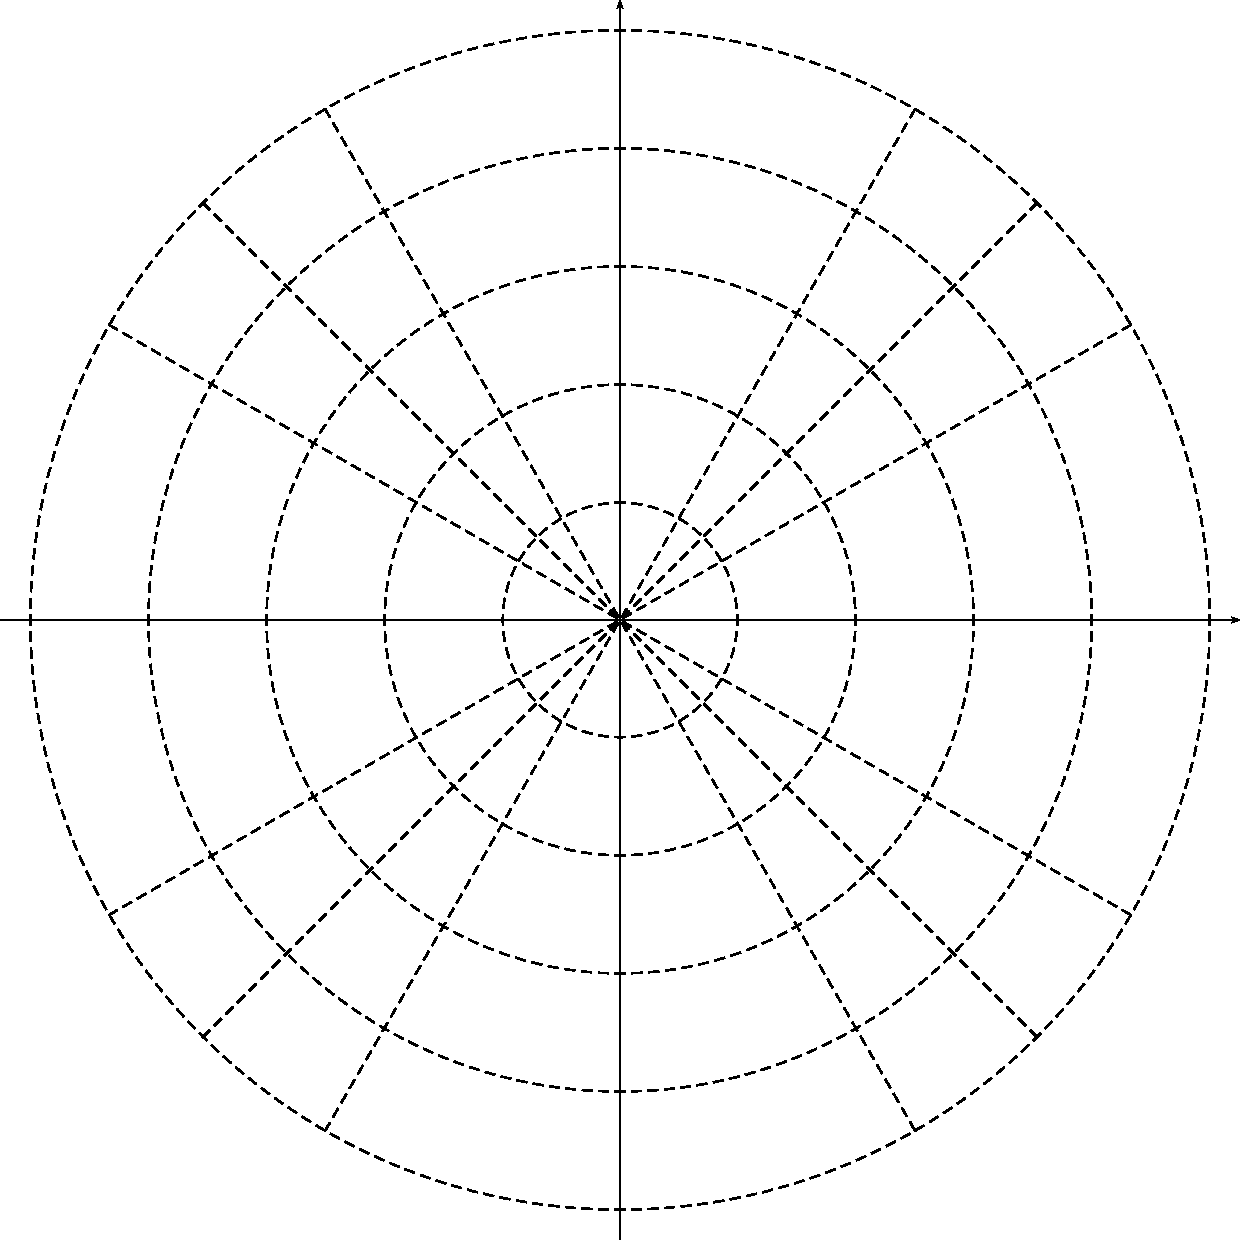
\includegraphics[width=0.5\linewidth]{resources/images/latex/grillepolaire} 

}

\caption{Grille polaire}\label{fig:grillepolaire}
\end{figure}

\BeginKnitrBlock{example}
\protect\hypertarget{exm:unnamed-chunk-102}{}{\label{exm:unnamed-chunk-102}
}Dessinez \(r=1=\sin(2\theta)\).
\EndKnitrBlock{example}

\begin{center}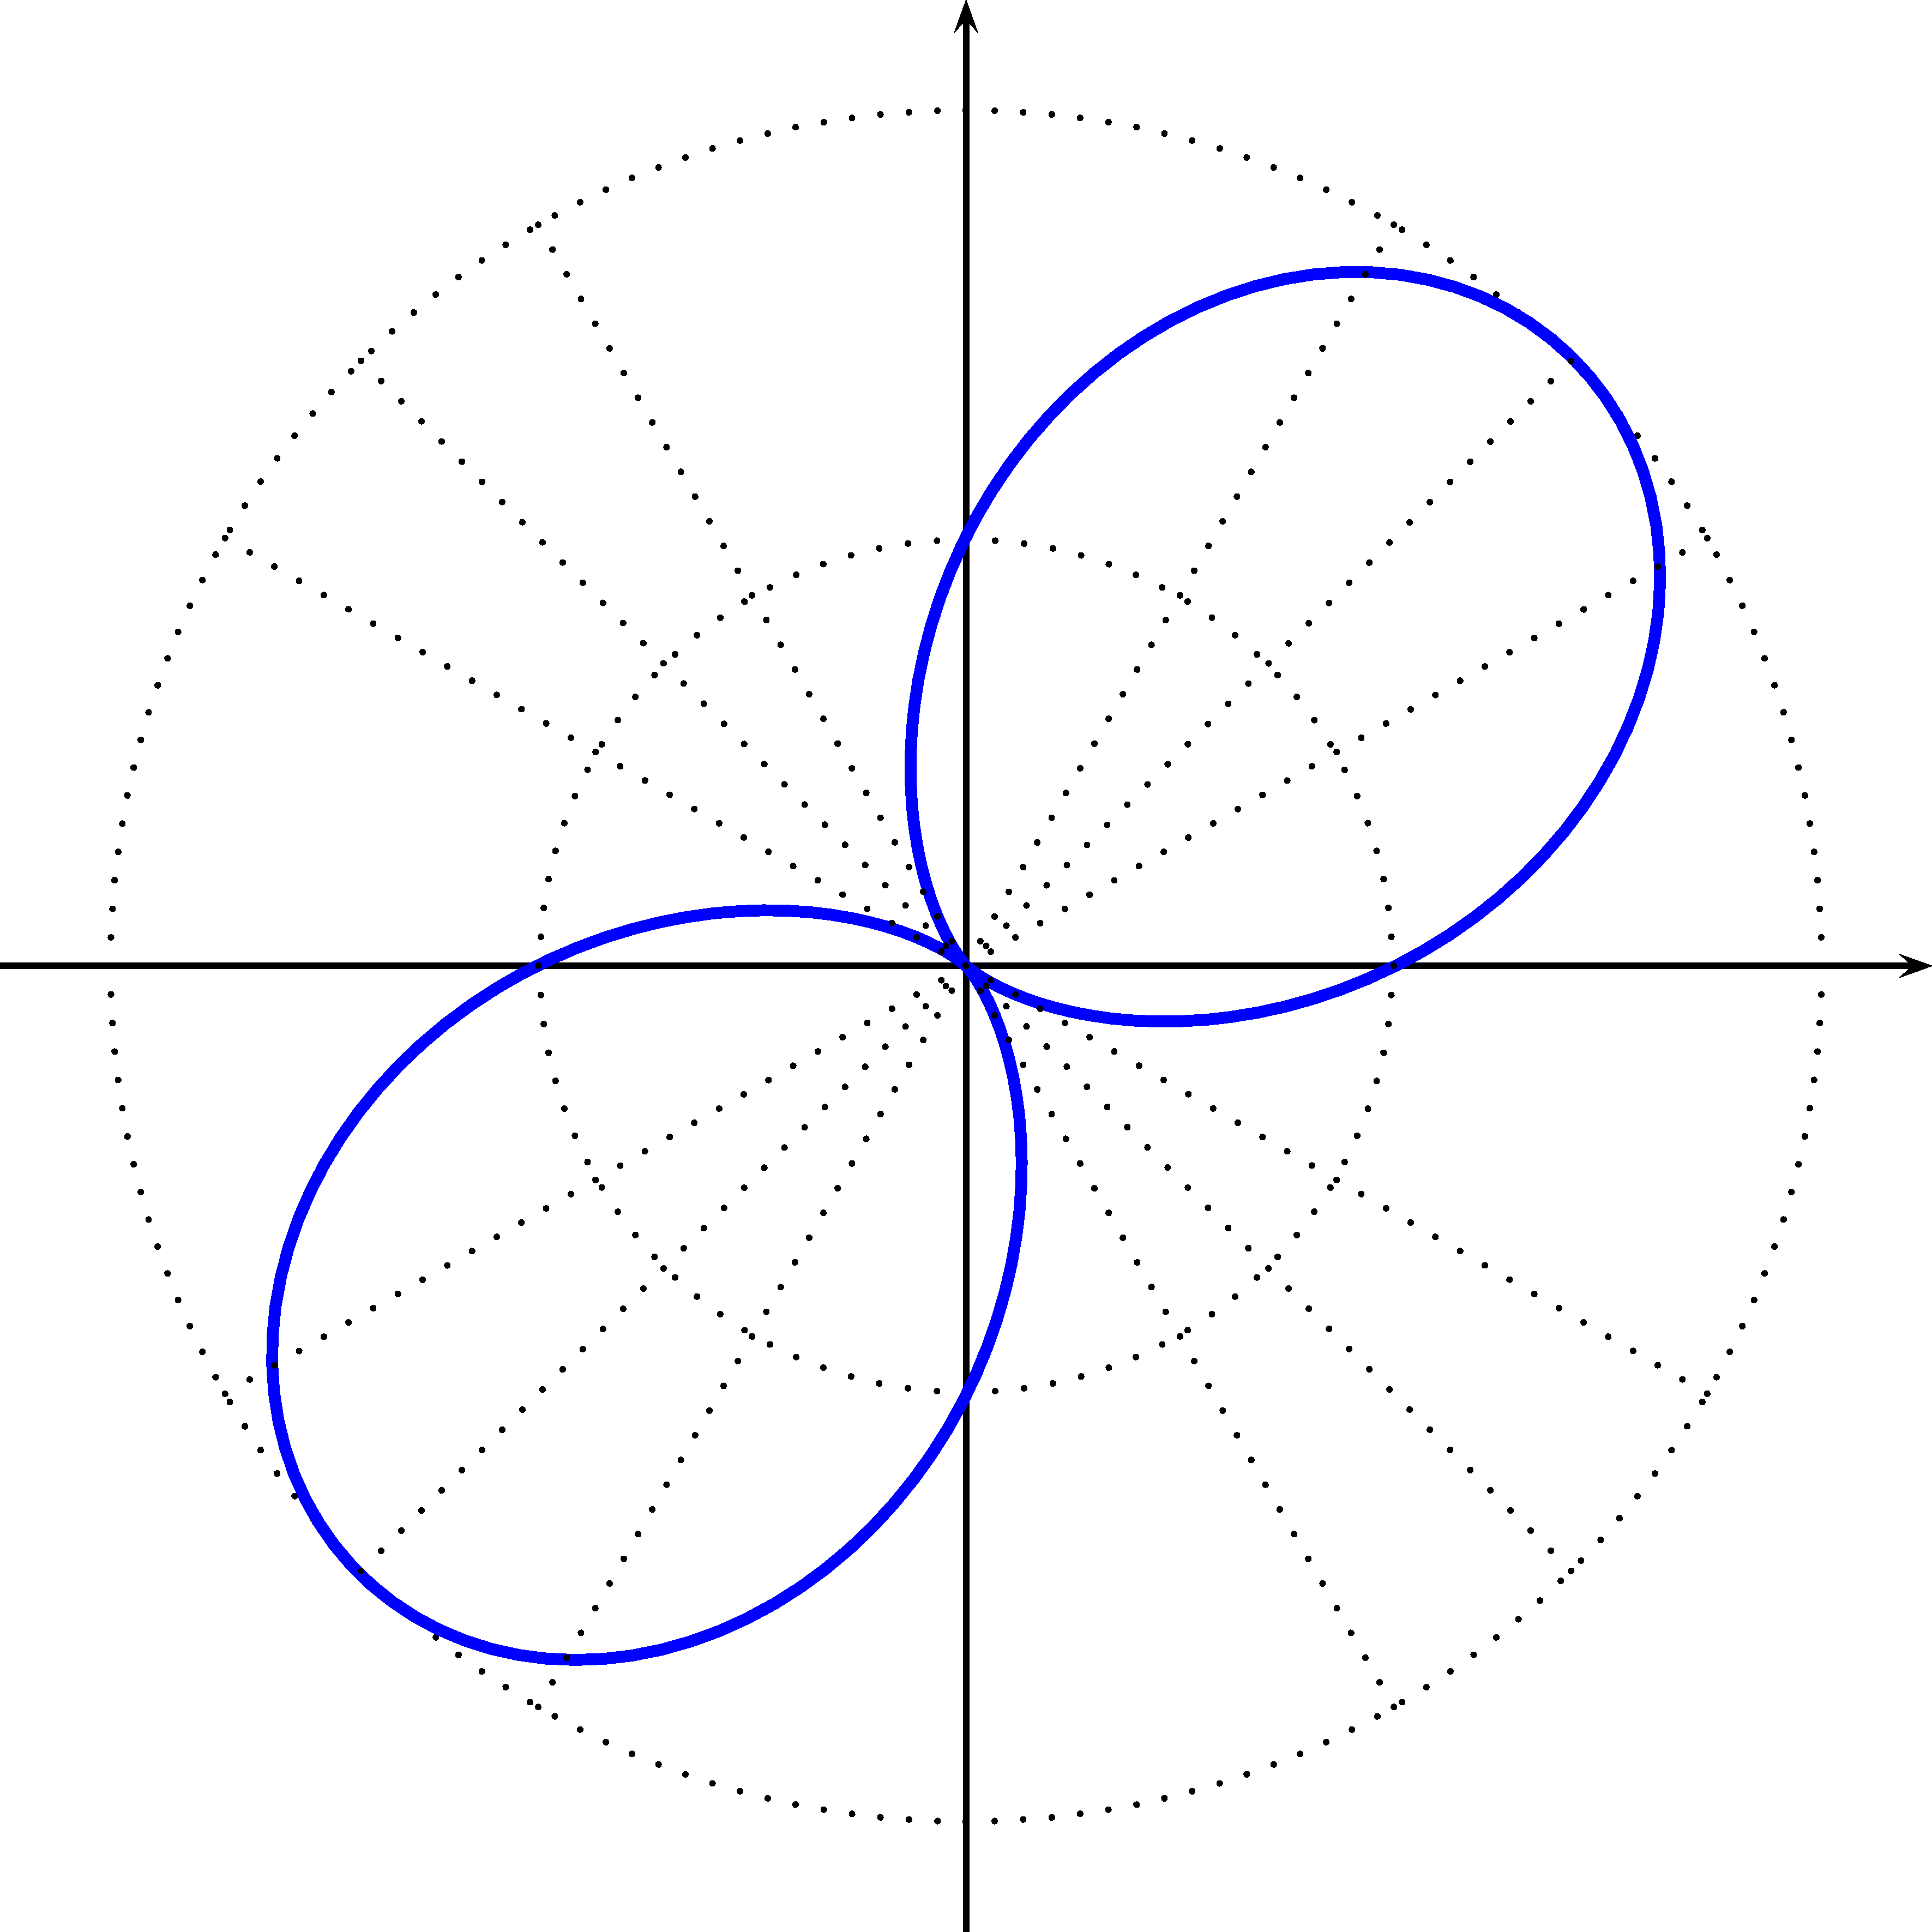
\includegraphics[width=0.5\linewidth]{resources/images/latex/ex1courbepolaire} \end{center}

\BeginKnitrBlock{example}
\protect\hypertarget{exm:unnamed-chunk-103}{}{\label{exm:unnamed-chunk-103}
}Dessinez \(r=1=\sin(\theta)\) pour \(\theta\in [0,2\pi]\).
\EndKnitrBlock{example}

\begin{center}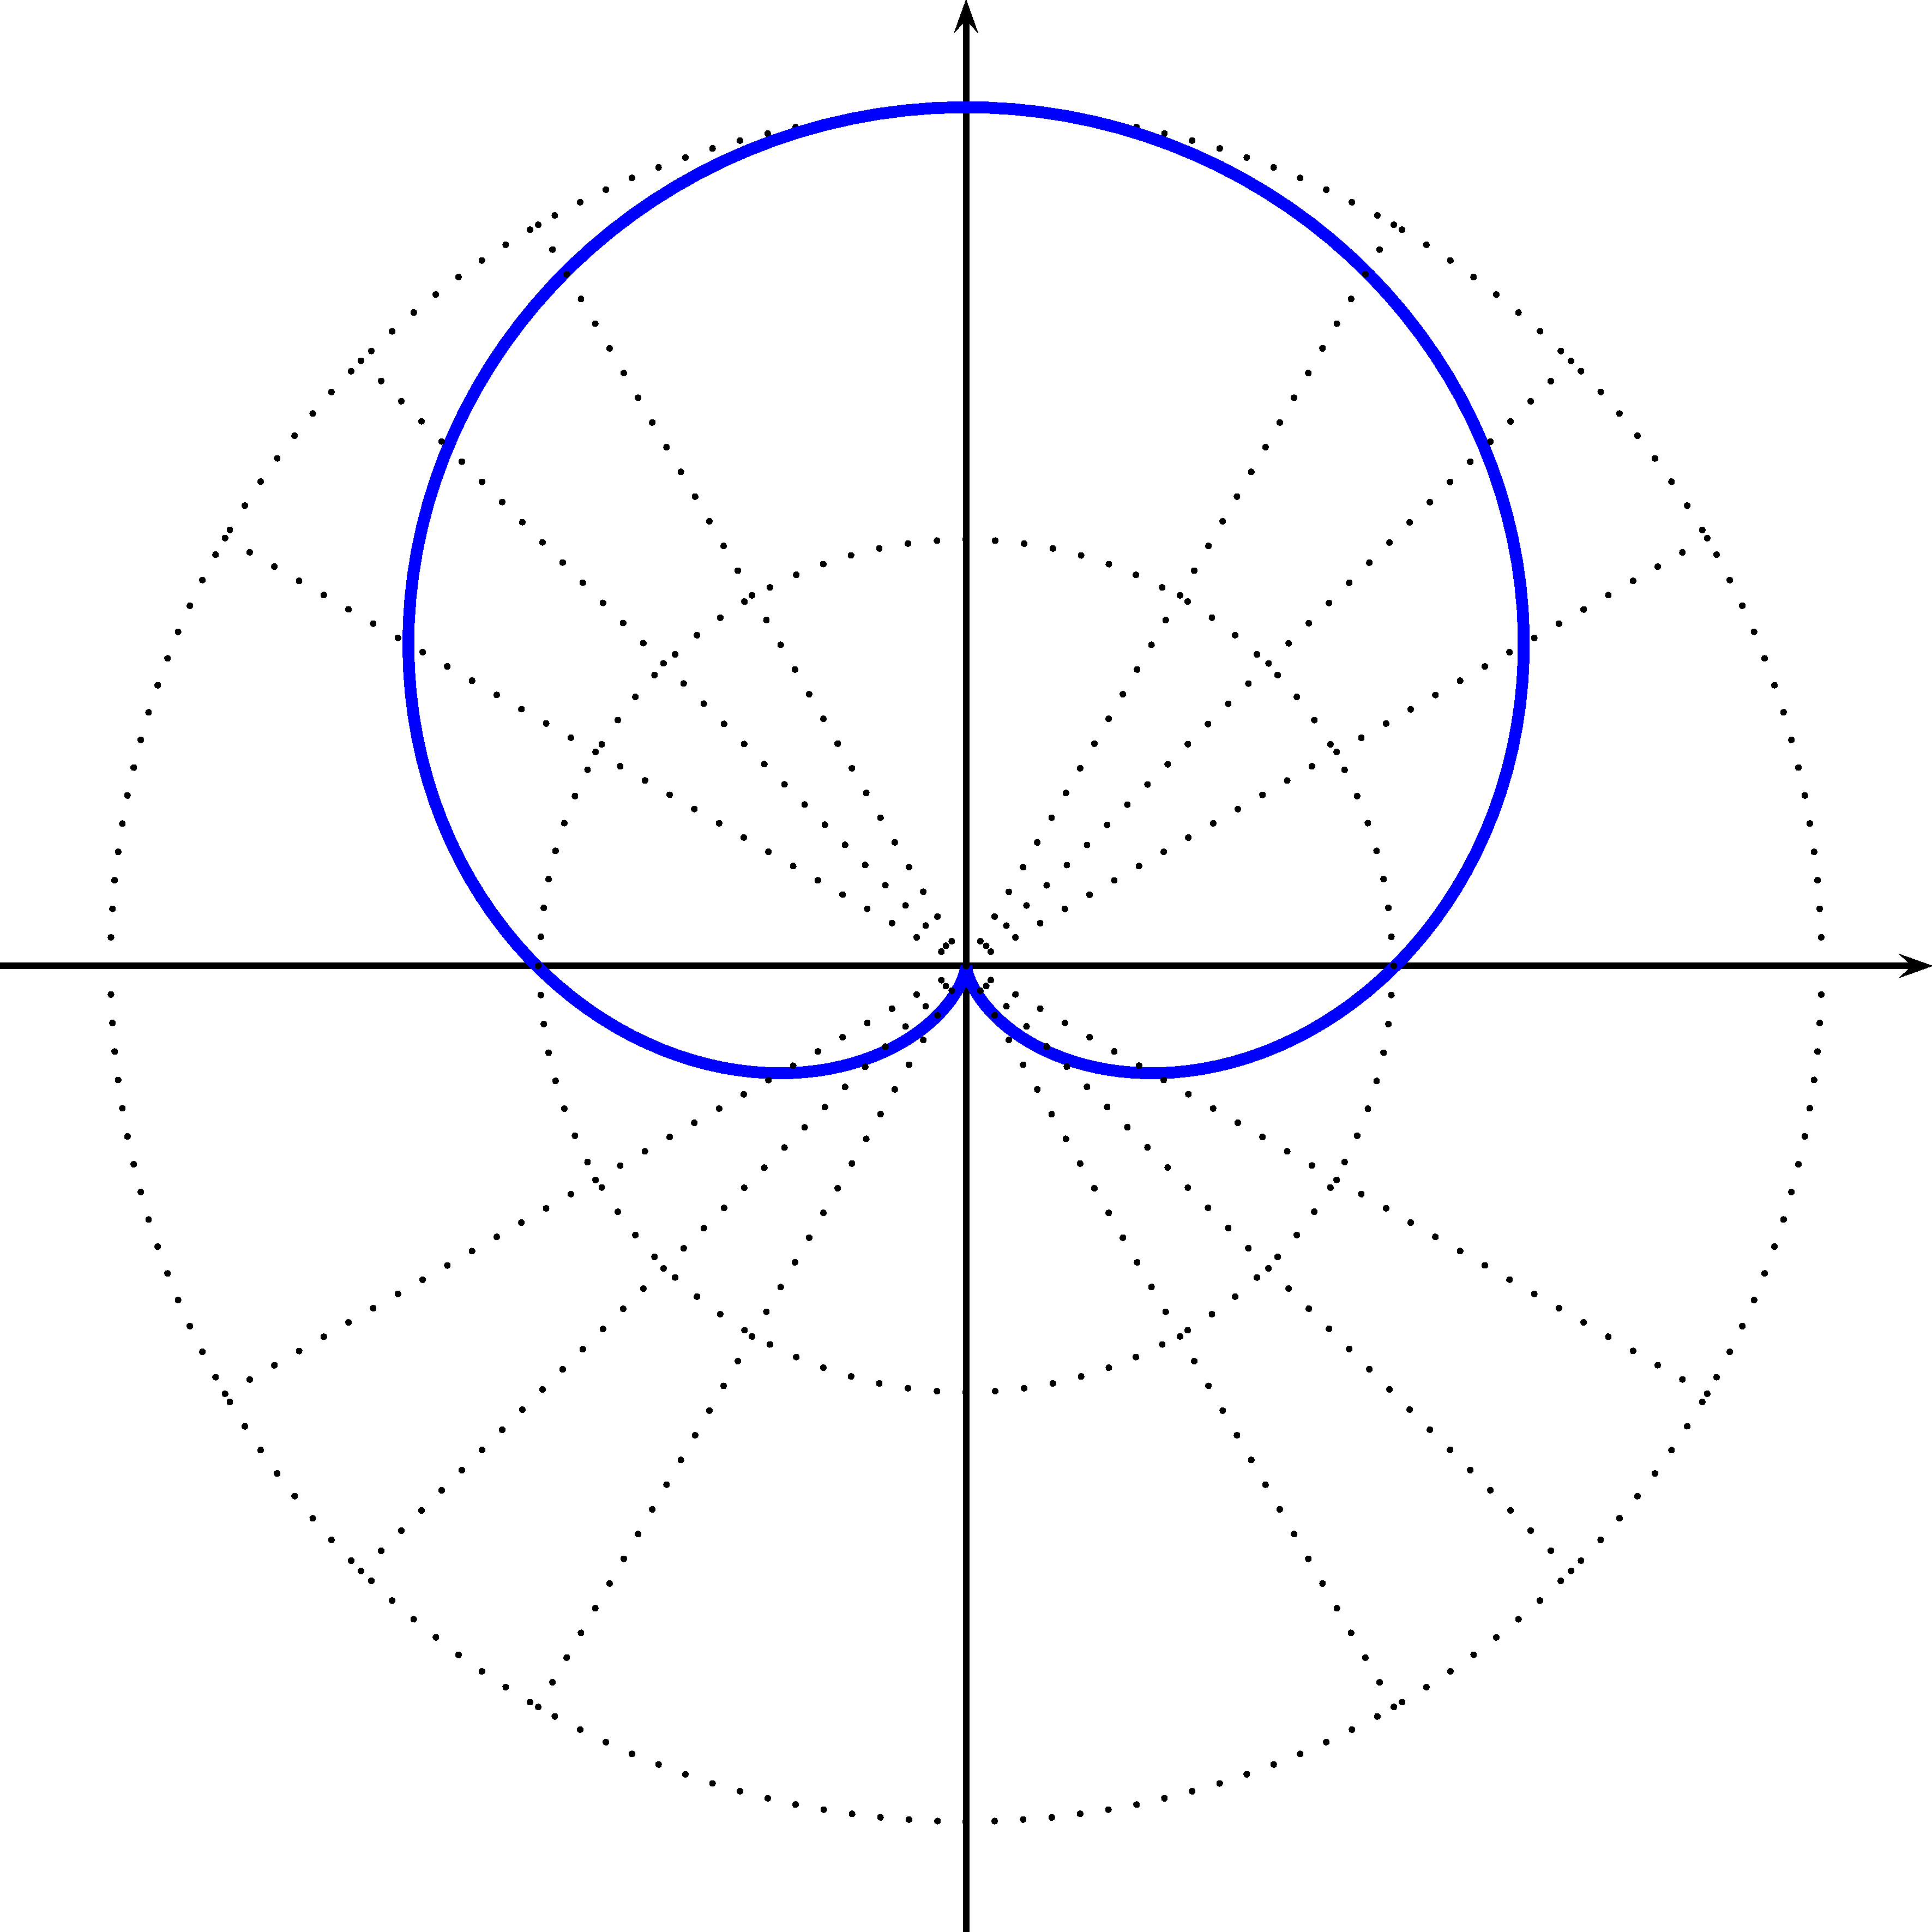
\includegraphics[width=0.5\linewidth]{resources/images/latex/ex2courbepolaire} \end{center}

\hypertarget{tangente-a-une-courbe-polaire}{%
\section{Tangente à une courbe
polaire}\label{tangente-a-une-courbe-polaire}}

Nous voulons maintenant déterminer les tangentes à des courbes polaires.
Nous savons que \(x=r\cos(\theta)\) et que \(y=r\sin(\theta)\). Si
\(r=f(\theta)\) alors nous avons que \(x=x(\theta)\) et \(y=y(\theta)\),
c'est-à-dire que \(x\) et \(y\) sont des fonctions de \(\theta\).

\BeginKnitrBlock{theorem}[Tangentes à une courbe polaire]
\protect\hypertarget{thm:unnamed-chunk-104}{}{\label{thm:unnamed-chunk-104}
\iffalse (Tangentes à une courbe polaire) \fi{} }Soit \(x\) et \(y\)
deux fonctions de \(\theta\). Si \(r=f(\theta)\), nous avons:
\begin{align*}
\dfrac{dy}{dx} &= \dfrac{f'(\theta)\sin(\theta)+f(\theta)\cos(\theta)}{f'(\theta)\cos(\theta)-f(\theta)\sin(\theta)}
\end{align*}
\EndKnitrBlock{theorem}

\BeginKnitrBlock{proof}
\iffalse{} {Preuve. } \fi{}Trouvons \(\dfrac{dx}{d\theta}\) et
\(\dfrac{dy}{d\theta}\). \begin{align*}
\dfrac{dx}{d\theta} &= \dfrac{d}{d\theta}\left[f(\theta)\cos(\theta)]\right] \\
&=  f'(\theta)\cos(\theta)-f(\theta)\sin(\theta) \\
\dfrac{dy}{d\theta} &= \dfrac{d}{d\theta}\left[f(\theta)\sin(\theta)]\right] \\
&=  f'(\theta)\sin(\theta)+f(\theta)\cos(\theta) 
\end{align*} Ainsi, \begin{align*}
\dfrac{dy}{dx} &= \dfrac{\dfrac{dy}{d\theta}}{\dfrac{dx}{d\theta}} \\
\dfrac{f'(\theta)\sin(\theta)+f(\theta)\cos(\theta)}{f'(\theta)\cos(\theta)-f(\theta)\sin(\theta)}
\end{align*}
\EndKnitrBlock{proof}

Nous avons maintenant une formule pour déterminer la pente de la droite
tangente.

\BeginKnitrBlock{example}
\protect\hypertarget{exm:unnamed-chunk-106}{}{\label{exm:unnamed-chunk-106}
}Trouvez l'équation de la droite tangente en \(\theta=\frac{\pi}{2}\) de
\(r=1+\sin(2\theta)\).
\EndKnitrBlock{example}
\vspace*{8cm}

\BeginKnitrBlock{example}
\protect\hypertarget{exm:unnamed-chunk-107}{}{\label{exm:unnamed-chunk-107}
}Soit l'équation \(r=2\cos(\theta)\).

\begin{enumerate}
\def\labelenumi{\alph{enumi}.}
\tightlist
\item
  Trouvez la dérivée \(\dfrac{dy}{dx}\).
\item
  Évaluez \(\left.\dfrac{dy}{dx}\right|_{\theta=\frac{\pi}{4}}\).
\item
  Évaluez \(\left.\dfrac{dy}{dx}\right|_{\theta=\frac{\pi}{3}}\).
\end{enumerate}
\EndKnitrBlock{example}
\vspace*{10cm}

\BeginKnitrBlock{example}
\protect\hypertarget{exm:unnamed-chunk-108}{}{\label{exm:unnamed-chunk-108}
}Trouvez la dérivée de la rose de Ghandi,
\(r=\cos\left(\dfrac{3\theta}{2}\right)\).
\EndKnitrBlock{example}
\vspace*{6cm}

\hypertarget{aire-dune-region}{%
\section{Aire d'une région}\label{aire-dune-region}}

Nous voulons maintenant trouver une formule afin de calculer l'aire
d'une région formée par une courbe définie par \(r=f(\theta)\) avec
\(\theta_a\leq \theta \leq \theta_b\).

Rappelons que l'aire \(A\) d'un secteur de cercle de rayon \(r\) est
donnée par \(A=\dfrac{1}{2}r^2\theta\).

La figure \ref{fig:airepolaire1} représente la surface que nous désirons
trouver.

\begin{figure}

{\centering 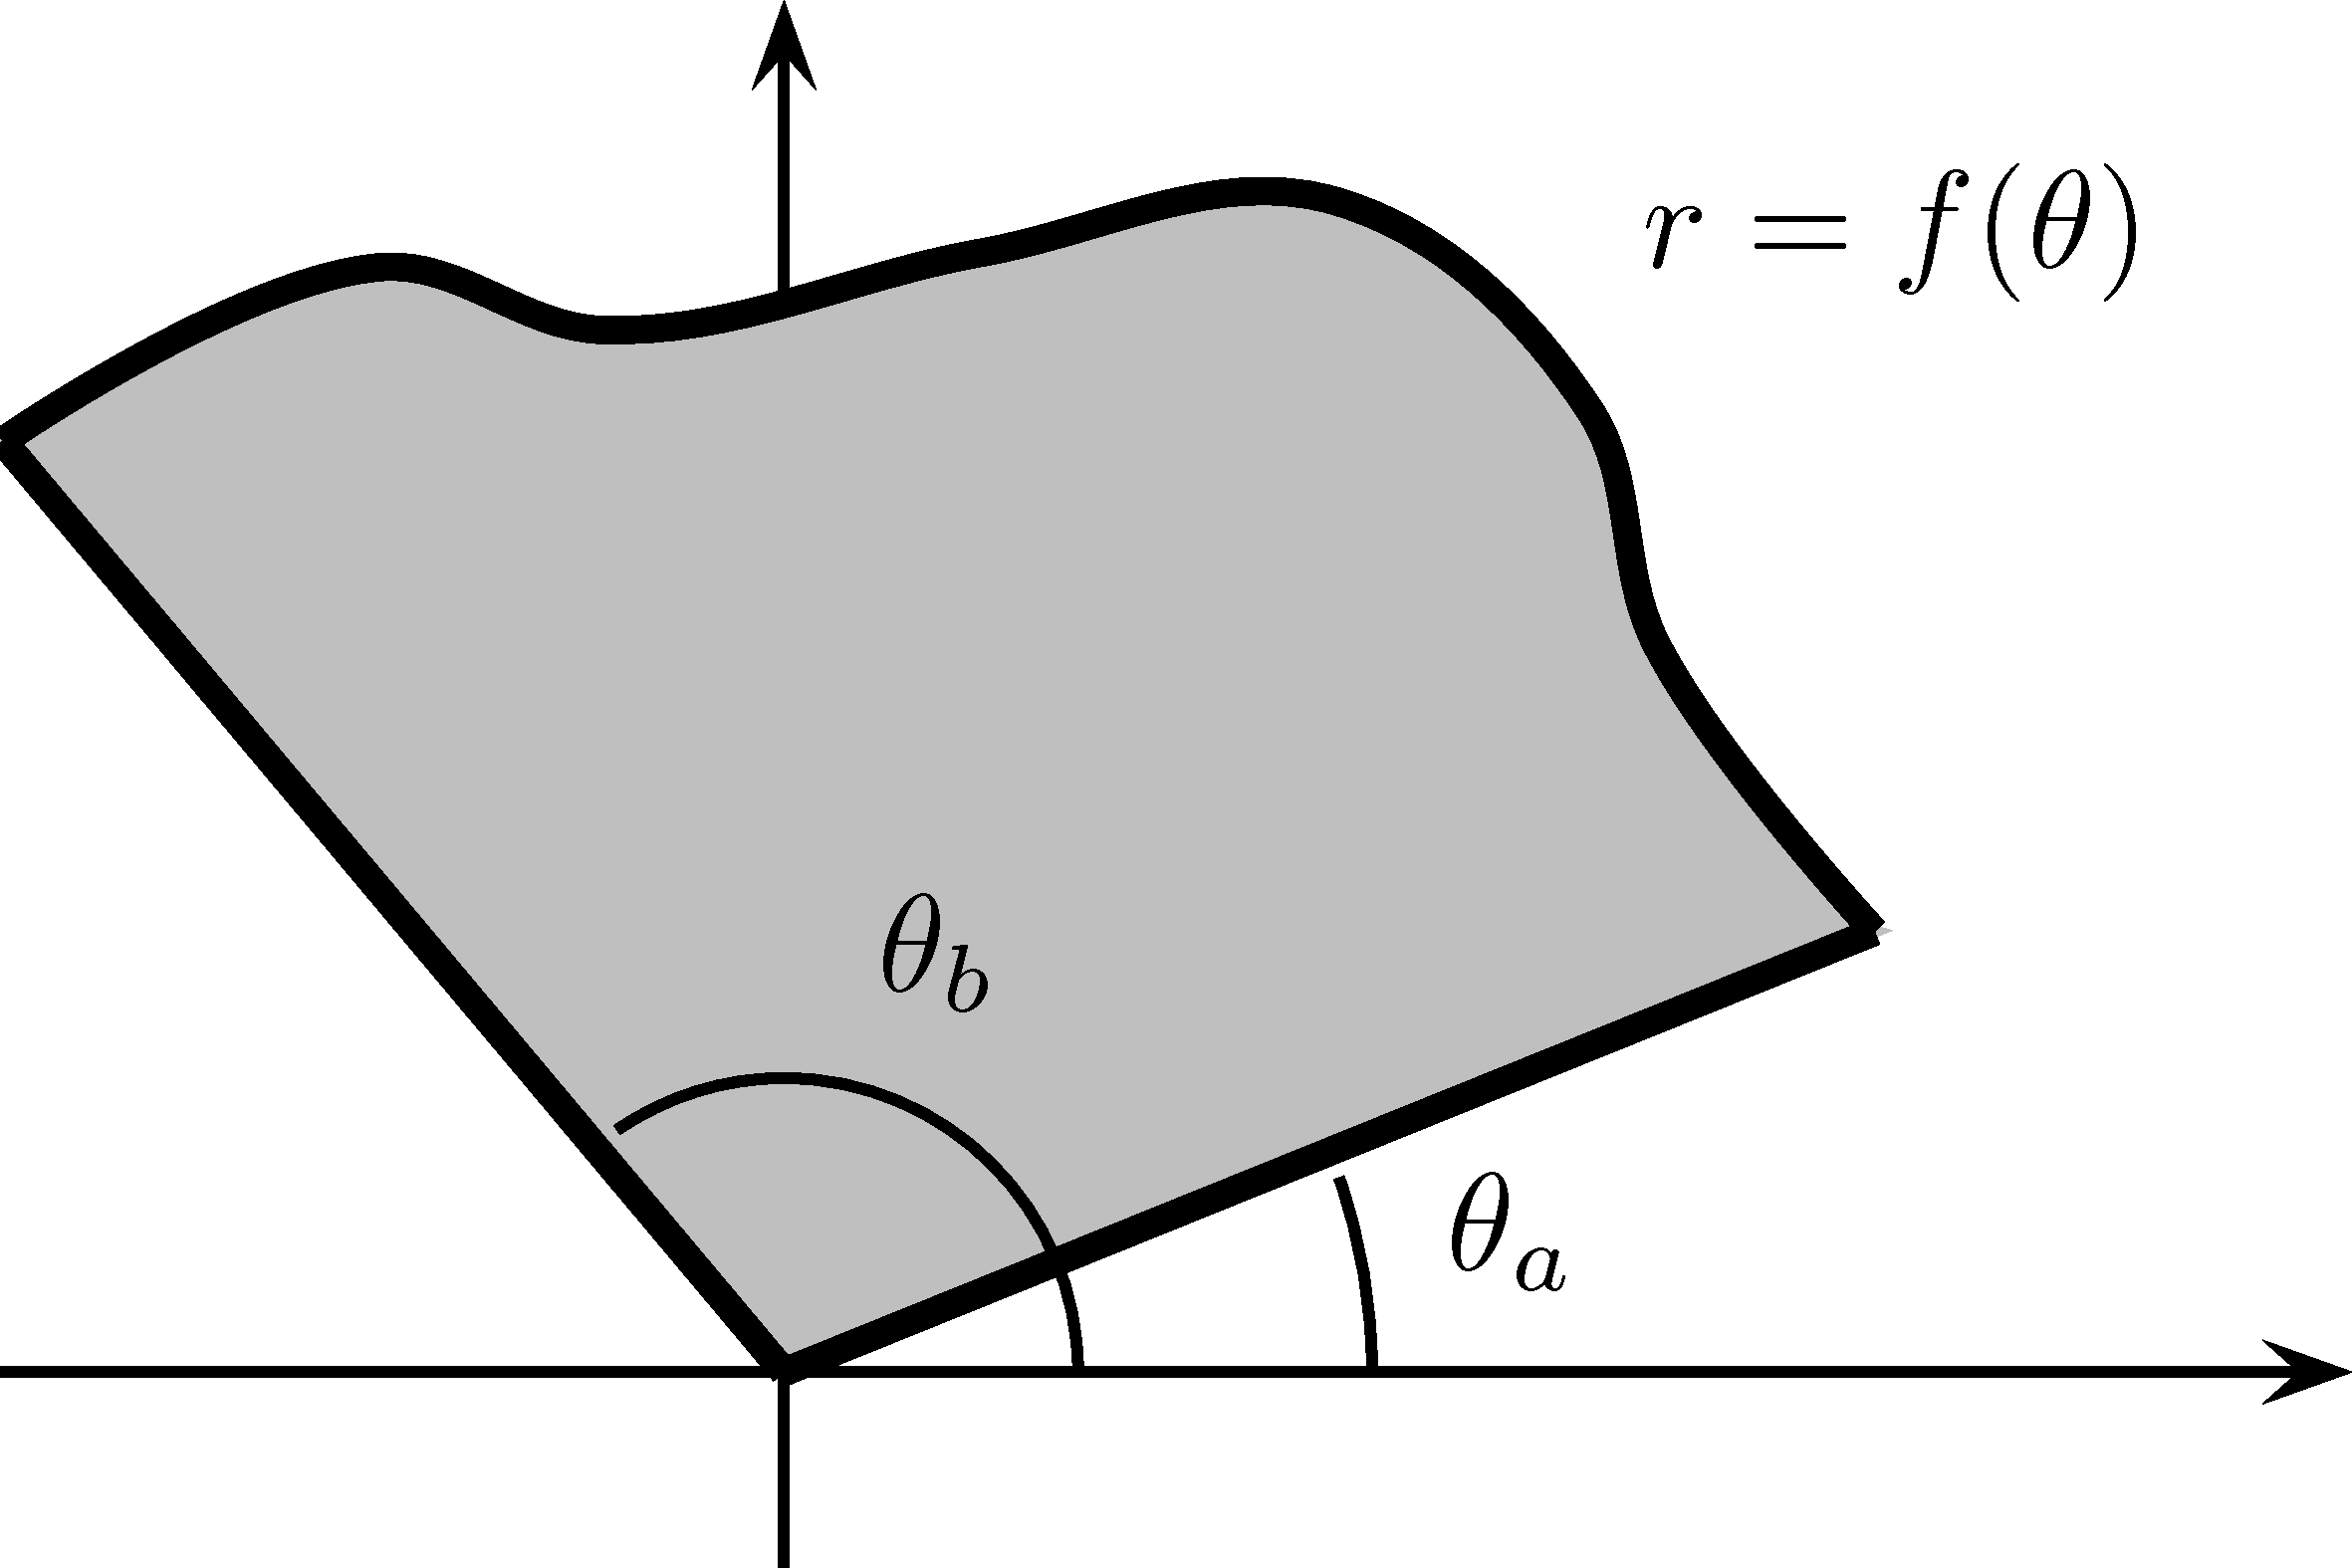
\includegraphics[width=0.5\linewidth]{resources/images/latex/airepolaire1} 

}

\caption{Aire d'une courbe polaire}\label{fig:airepolaire1}
\end{figure}

Divisons l'intervalle \(\theta_a\leq \theta \leq \theta_b\) en \(N\)
partitions de longueur \(\Delta \theta_i=\theta_i-\theta_{i-1}\) pour
\(i=1,\ldots,N\). L'ensemble \begin{align*}
\{\theta_0=\theta_a,\theta_1,...,\theta_{N-1},\theta_{N}=\theta_b\}
\end{align*} est appelée partition de
\(\theta_a\leq \theta \leq \theta_b\). L'aire de chacun de ces secteurs
peut être approchée par: \begin{align*}
A_i\approx \dfrac{1}{2}[f(\theta_i^*)]^2\Delta \theta_i, \quad \text{où $\theta_i^*\in [\theta_{i-1},\theta_{i}]$}
\end{align*}

La figure \ref{fig:airepolaire2} représente une partition.

\begin{figure}

{\centering 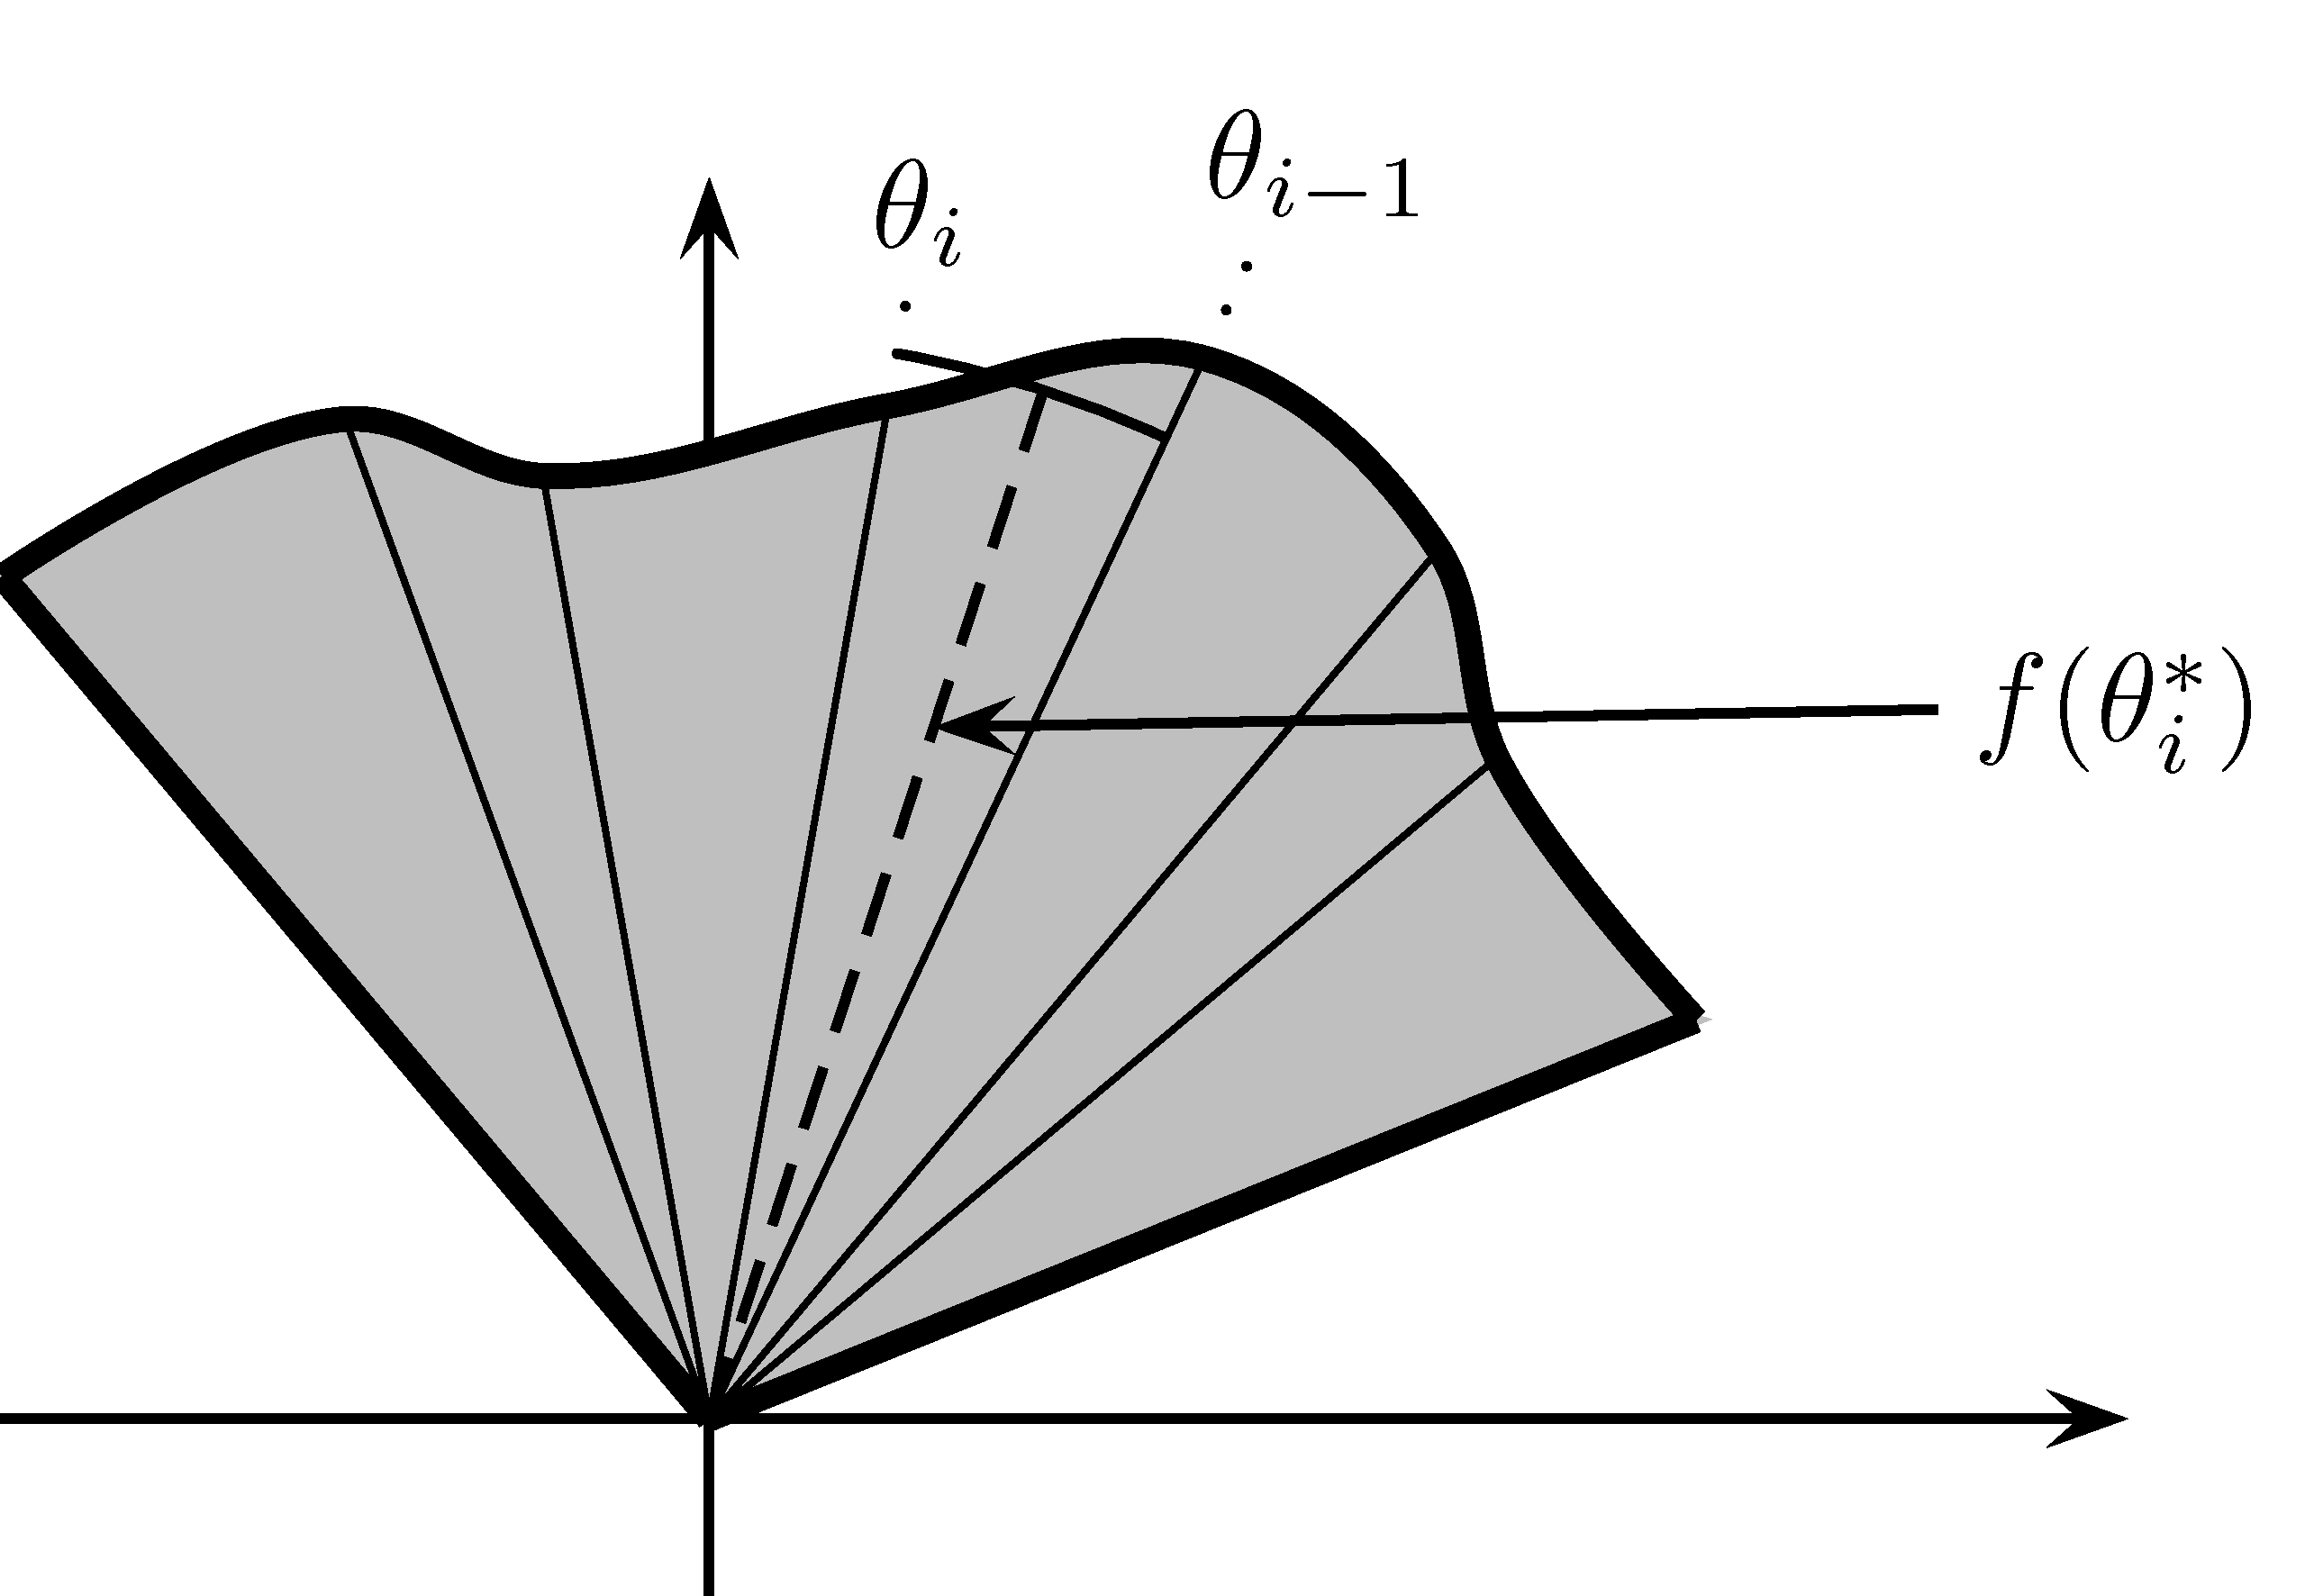
\includegraphics[width=0.5\linewidth]{resources/images/latex/airepolaire2} 

}

\caption{Aire d'une courbe polaire: séparation en secteurs}\label{fig:airepolaire2}
\end{figure}

Nous voulons trouver l'aire totale, c'est-à-dire la somme des surfaces
des \(N\) secteurs: \begin{align*}
A\approx \sum_{i=1}^N\dfrac{1}{2}[f(\theta_i^*)]^2\Delta \theta_i
\end{align*} Nous remarquons que cette somme est une somme de Riemann.
Ainsi, en prenant la limite lorsque \(N\) tend vers l'infini, nous
obtenons: \begin{align*}
A=\lim_{N\rightarrow \infty } \sum_{i=1}^N\dfrac{1}{2}[f(\theta_i^*)]^2\Delta \theta_i=\int_{\theta_a}^{\theta_b}\dfrac{1}{2}[f(\theta)]^2d \theta
\end{align*}

D'où, l'aire est donnée par: \begin{align*}
A &= \int_{\theta_a}^{\theta_b}\dfrac{1}{2}[f(\theta)]^2 d\theta
\end{align*}

\BeginKnitrBlock{example}
\protect\hypertarget{exm:unnamed-chunk-109}{}{\label{exm:unnamed-chunk-109}
}Calculez l'aire de la région formée par \(r=1+\sin(2\theta)\).
\EndKnitrBlock{example}

\begin{center}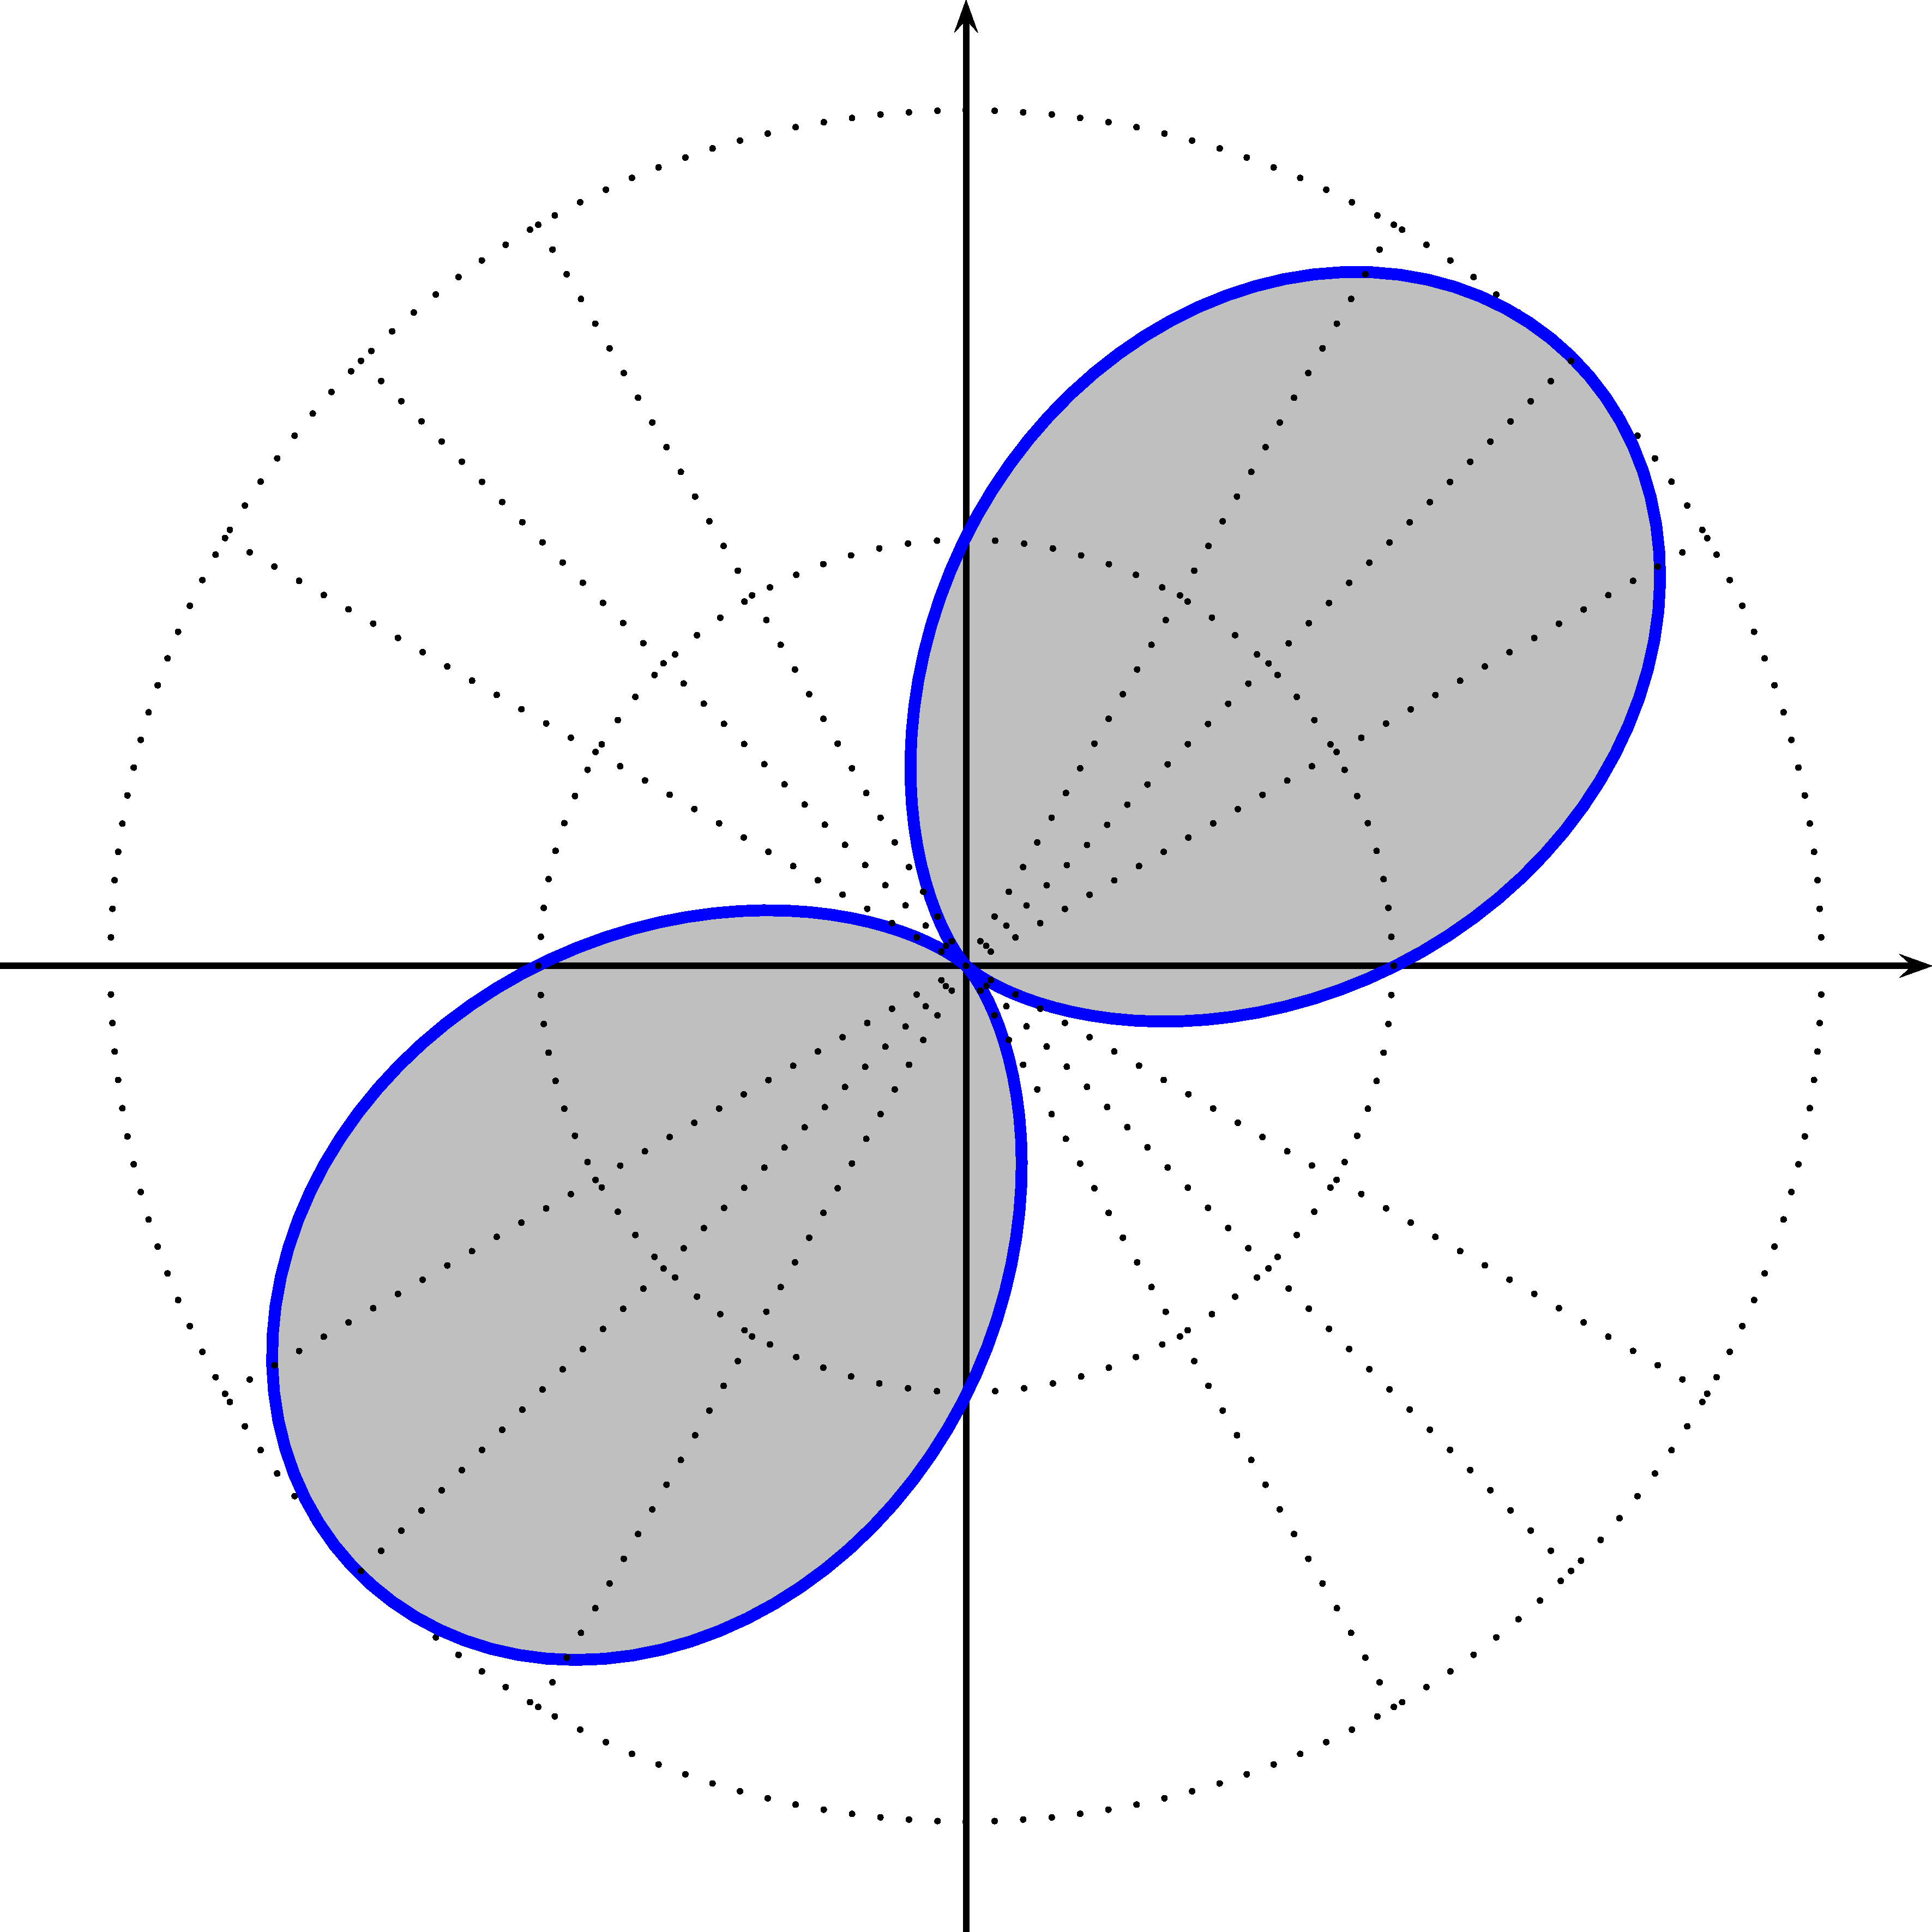
\includegraphics[width=0.5\linewidth]{resources/images/latex/ex1airepolaire} \end{center}
\vspace*{10cm}

\BeginKnitrBlock{example}
\protect\hypertarget{exm:unnamed-chunk-110}{}{\label{exm:unnamed-chunk-110}
}Calculez l'aire située au-dessus du cercle \(r=3\sin(\theta)\) et en
dessous de la cardioïde \(r=1+\sin(\theta)\).
\EndKnitrBlock{example}

\begin{center}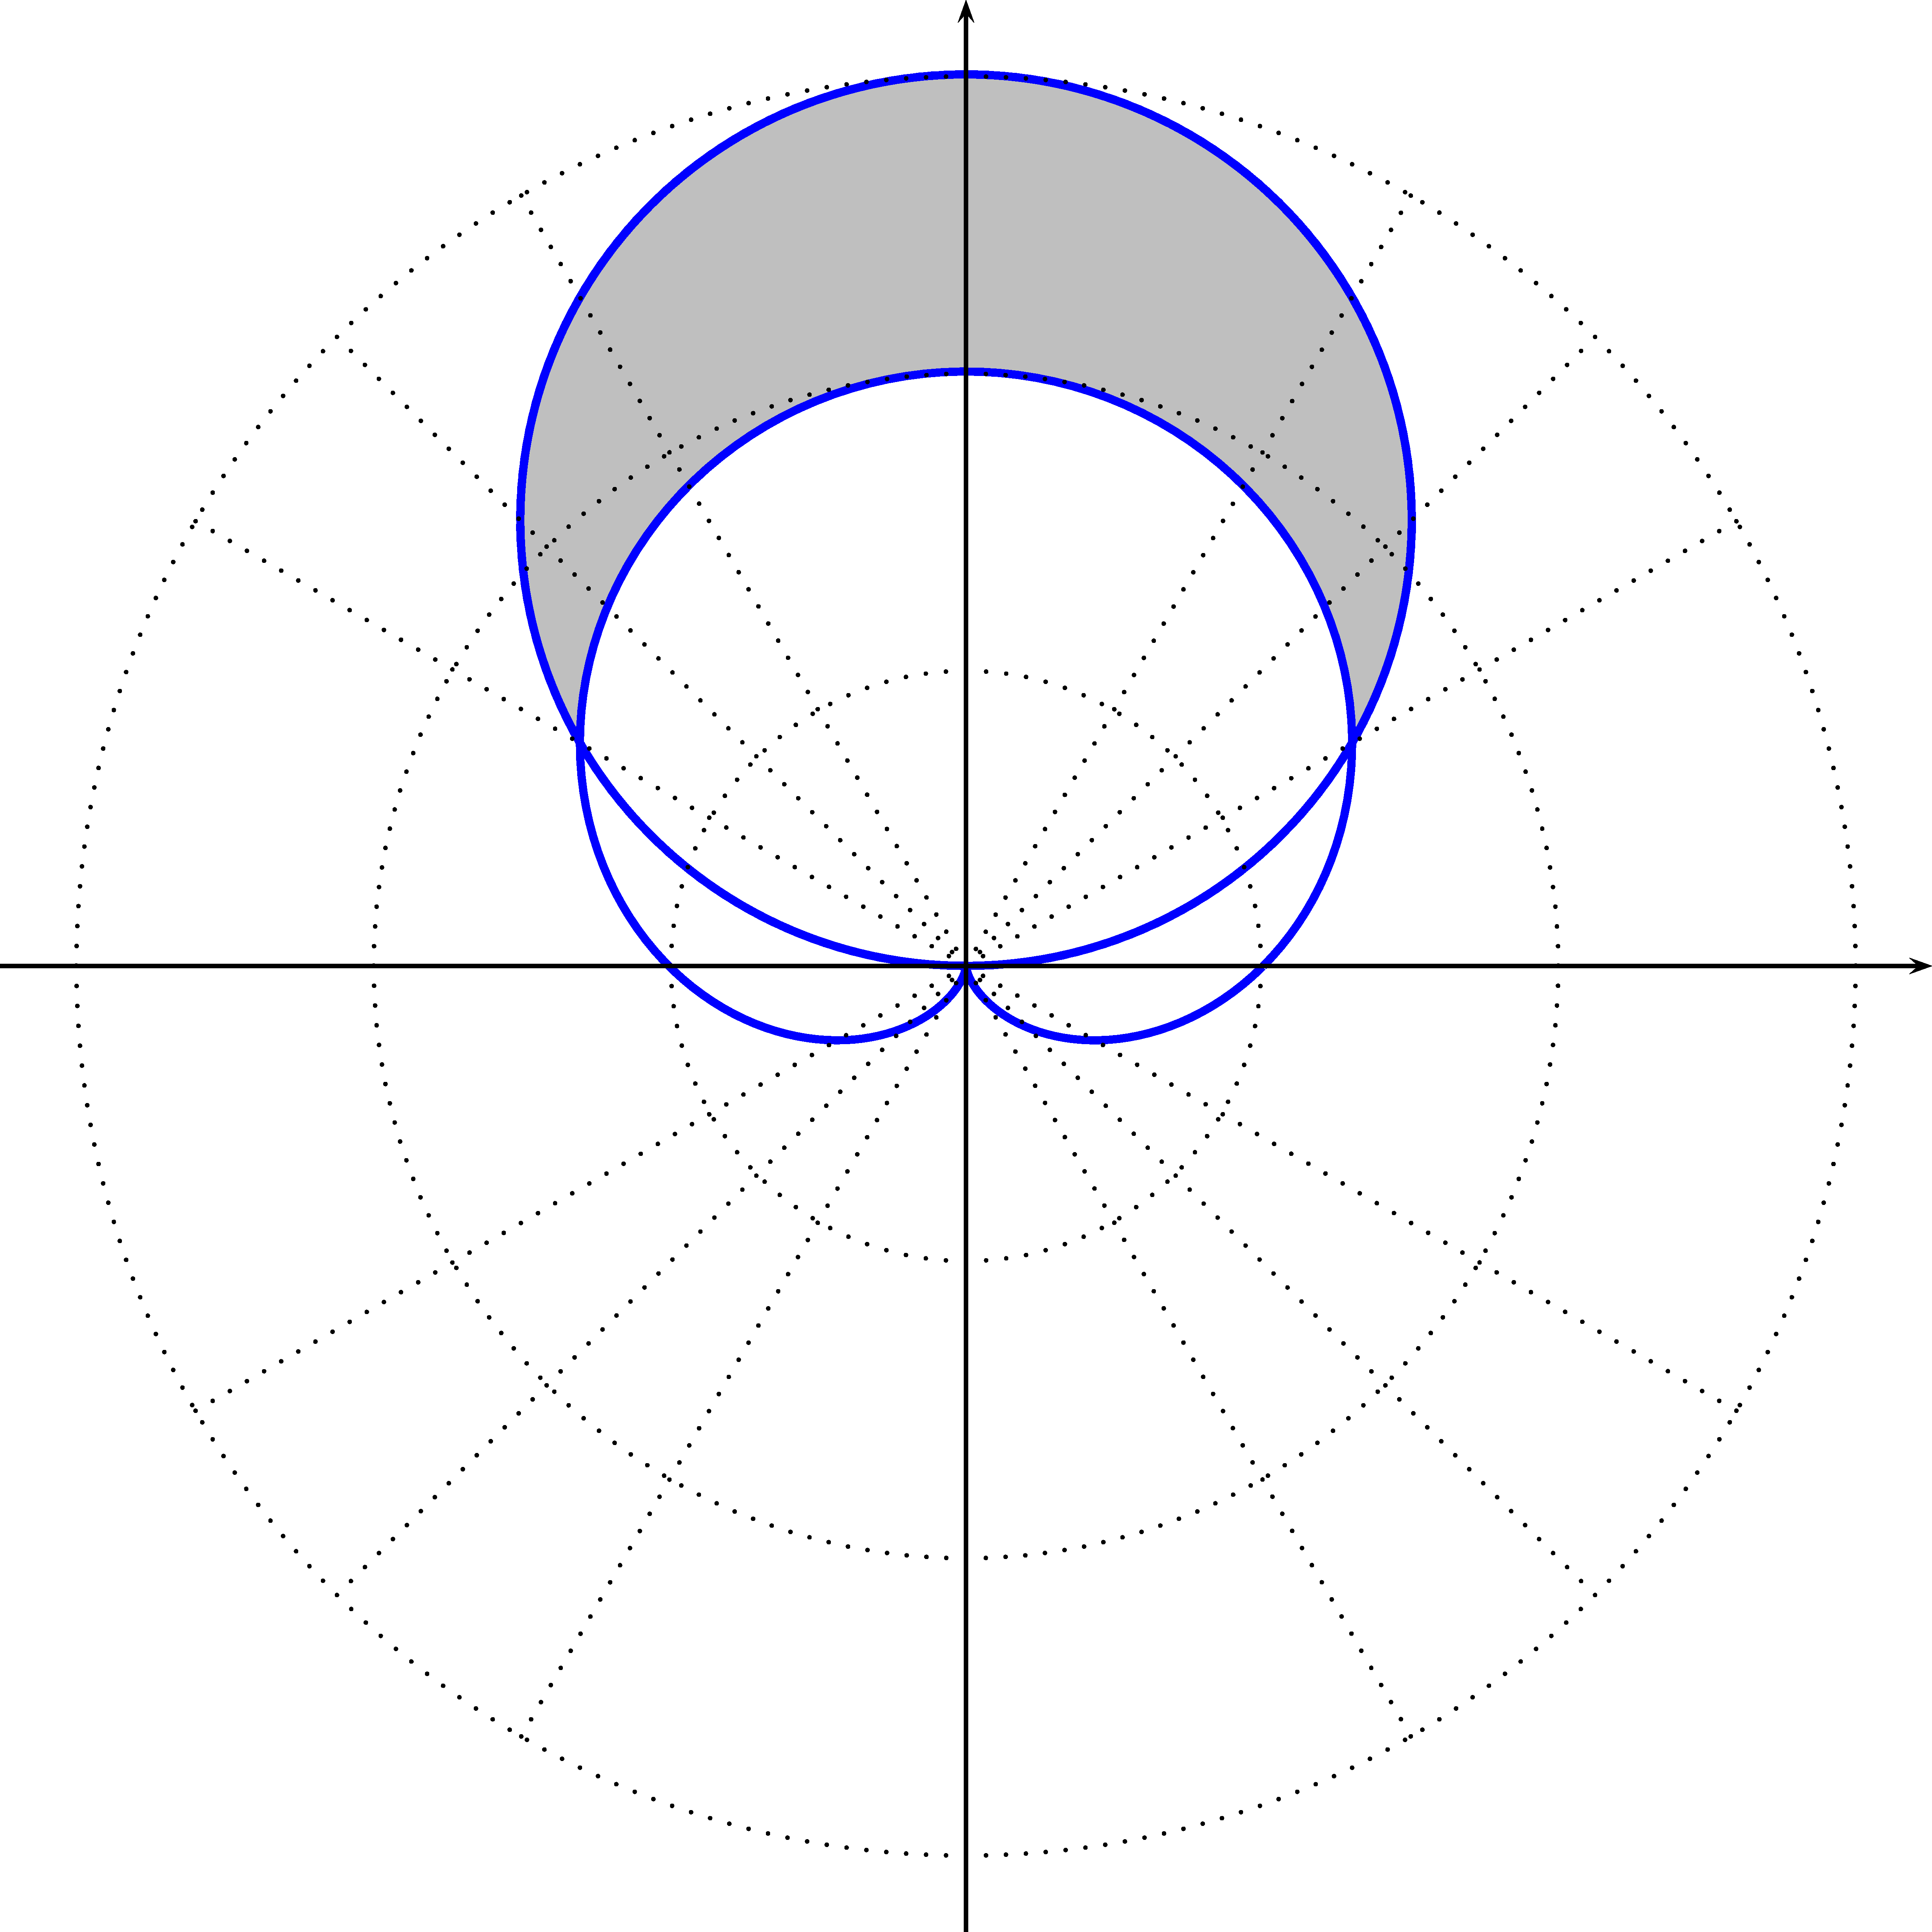
\includegraphics[width=0.5\linewidth]{resources/images/latex/ex2airepolaire} \end{center}
\vspace*{10cm}

\BeginKnitrBlock{example}
\protect\hypertarget{exm:unnamed-chunk-111}{}{\label{exm:unnamed-chunk-111}
}Calculez l'aire d'une seule feuille de \(r=1+\sin(\theta)\) avec
\(0\leq \theta \leq \frac{\pi}{3}\).
\EndKnitrBlock{example}
\vspace*{10cm}

\BeginKnitrBlock{example}
\protect\hypertarget{exm:unnamed-chunk-112}{}{\label{exm:unnamed-chunk-112}
}Calculez l'aire du quadrifolium \(r=\cos(2\theta)\) si un seul pétale
se trouve dans l'intervalle
\(\frac{\pi}{4}\leq \theta \leq \frac{3\pi}{4}\).
\EndKnitrBlock{example}
\vspace*{10cm}

\hypertarget{longueur-dune-courbe}{%
\section{Longueur d'une courbe}\label{longueur-dune-courbe}}

\BeginKnitrBlock{theorem}[Logueur d'une courbe en coordonnées polaires]
\protect\hypertarget{thm:unnamed-chunk-113}{}{\label{thm:unnamed-chunk-113}
\iffalse (Logueur d'une courbe en coordonnées polaires) \fi{} }La
longueur d'une courbe en coordonnées polaires définie par
\(r=f(\theta)\) où \(\theta_a\leq\theta\leq\theta_b\) est donnée par:
\begin{align*}
L=\int_{\theta_a}^{\theta_b}\sqrt{\left(\dfrac{dr}{d\theta}\right)^2+r^2}d\theta
\end{align*}
\EndKnitrBlock{theorem}

\BeginKnitrBlock{proof}
\iffalse{} {Preuve. } \fi{}La démonstration suivante escamote plusieurs
utilisations des sommes de Riemann pour simplifier.

Nous savons que: \begin{align*}
L &= \int_a^b \sqrt{1+\left(\dfrac{dy}{dx}\right)^2}dx \\
&= \int_a^b \sqrt{(dx)^2\left(1+\left(\dfrac{dy}{dx}\right)^2\right)} \\
&= \int_a^b \sqrt{(dx)^2+(dy)^2} \\
&= 
\end{align*}
\EndKnitrBlock{proof}

La longueur d'une courbe en coordonnées polaires définie par
\(r=f(\theta)\)

\hypertarget{geogebra-polaire}{%
\section{GeoGebra}\label{geogebra-polaire}}

\hypertarget{applet_container}{}

\hypertarget{fctvar}{%
\chapter{Les fonctions de plusieurs variables}\label{fctvar}}

\hypertarget{intfct}{%
\chapter{L'intégration de fonctions de plusieurs
variables}\label{intfct}}

\bibliography{book.bib,packages.bib}


\end{document}
